% Options for packages loaded elsewhere
\PassOptionsToPackage{unicode}{hyperref}
\PassOptionsToPackage{hyphens}{url}
%
\documentclass[
]{article}
\usepackage{amsmath,amssymb}
\usepackage{iftex}
\ifPDFTeX
  \usepackage[T1]{fontenc}
  \usepackage[utf8]{inputenc}
  \usepackage{textcomp} % provide euro and other symbols
\else % if luatex or xetex
  \usepackage{unicode-math} % this also loads fontspec
  \defaultfontfeatures{Scale=MatchLowercase}
  \defaultfontfeatures[\rmfamily]{Ligatures=TeX,Scale=1}
\fi
\usepackage{lmodern}
\ifPDFTeX\else
  % xetex/luatex font selection
\fi
% Use upquote if available, for straight quotes in verbatim environments
\IfFileExists{upquote.sty}{\usepackage{upquote}}{}
\IfFileExists{microtype.sty}{% use microtype if available
  \usepackage[]{microtype}
  \UseMicrotypeSet[protrusion]{basicmath} % disable protrusion for tt fonts
}{}
\makeatletter
\@ifundefined{KOMAClassName}{% if non-KOMA class
  \IfFileExists{parskip.sty}{%
    \usepackage{parskip}
  }{% else
    \setlength{\parindent}{0pt}
    \setlength{\parskip}{6pt plus 2pt minus 1pt}}
}{% if KOMA class
  \KOMAoptions{parskip=half}}
\makeatother
\usepackage{xcolor}
\usepackage[margin=1in]{geometry}
\usepackage{color}
\usepackage{fancyvrb}
\newcommand{\VerbBar}{|}
\newcommand{\VERB}{\Verb[commandchars=\\\{\}]}
\DefineVerbatimEnvironment{Highlighting}{Verbatim}{commandchars=\\\{\}}
% Add ',fontsize=\small' for more characters per line
\usepackage{framed}
\definecolor{shadecolor}{RGB}{248,248,248}
\newenvironment{Shaded}{\begin{snugshade}}{\end{snugshade}}
\newcommand{\AlertTok}[1]{\textcolor[rgb]{0.94,0.16,0.16}{#1}}
\newcommand{\AnnotationTok}[1]{\textcolor[rgb]{0.56,0.35,0.01}{\textbf{\textit{#1}}}}
\newcommand{\AttributeTok}[1]{\textcolor[rgb]{0.13,0.29,0.53}{#1}}
\newcommand{\BaseNTok}[1]{\textcolor[rgb]{0.00,0.00,0.81}{#1}}
\newcommand{\BuiltInTok}[1]{#1}
\newcommand{\CharTok}[1]{\textcolor[rgb]{0.31,0.60,0.02}{#1}}
\newcommand{\CommentTok}[1]{\textcolor[rgb]{0.56,0.35,0.01}{\textit{#1}}}
\newcommand{\CommentVarTok}[1]{\textcolor[rgb]{0.56,0.35,0.01}{\textbf{\textit{#1}}}}
\newcommand{\ConstantTok}[1]{\textcolor[rgb]{0.56,0.35,0.01}{#1}}
\newcommand{\ControlFlowTok}[1]{\textcolor[rgb]{0.13,0.29,0.53}{\textbf{#1}}}
\newcommand{\DataTypeTok}[1]{\textcolor[rgb]{0.13,0.29,0.53}{#1}}
\newcommand{\DecValTok}[1]{\textcolor[rgb]{0.00,0.00,0.81}{#1}}
\newcommand{\DocumentationTok}[1]{\textcolor[rgb]{0.56,0.35,0.01}{\textbf{\textit{#1}}}}
\newcommand{\ErrorTok}[1]{\textcolor[rgb]{0.64,0.00,0.00}{\textbf{#1}}}
\newcommand{\ExtensionTok}[1]{#1}
\newcommand{\FloatTok}[1]{\textcolor[rgb]{0.00,0.00,0.81}{#1}}
\newcommand{\FunctionTok}[1]{\textcolor[rgb]{0.13,0.29,0.53}{\textbf{#1}}}
\newcommand{\ImportTok}[1]{#1}
\newcommand{\InformationTok}[1]{\textcolor[rgb]{0.56,0.35,0.01}{\textbf{\textit{#1}}}}
\newcommand{\KeywordTok}[1]{\textcolor[rgb]{0.13,0.29,0.53}{\textbf{#1}}}
\newcommand{\NormalTok}[1]{#1}
\newcommand{\OperatorTok}[1]{\textcolor[rgb]{0.81,0.36,0.00}{\textbf{#1}}}
\newcommand{\OtherTok}[1]{\textcolor[rgb]{0.56,0.35,0.01}{#1}}
\newcommand{\PreprocessorTok}[1]{\textcolor[rgb]{0.56,0.35,0.01}{\textit{#1}}}
\newcommand{\RegionMarkerTok}[1]{#1}
\newcommand{\SpecialCharTok}[1]{\textcolor[rgb]{0.81,0.36,0.00}{\textbf{#1}}}
\newcommand{\SpecialStringTok}[1]{\textcolor[rgb]{0.31,0.60,0.02}{#1}}
\newcommand{\StringTok}[1]{\textcolor[rgb]{0.31,0.60,0.02}{#1}}
\newcommand{\VariableTok}[1]{\textcolor[rgb]{0.00,0.00,0.00}{#1}}
\newcommand{\VerbatimStringTok}[1]{\textcolor[rgb]{0.31,0.60,0.02}{#1}}
\newcommand{\WarningTok}[1]{\textcolor[rgb]{0.56,0.35,0.01}{\textbf{\textit{#1}}}}
\usepackage{graphicx}
\makeatletter
\def\maxwidth{\ifdim\Gin@nat@width>\linewidth\linewidth\else\Gin@nat@width\fi}
\def\maxheight{\ifdim\Gin@nat@height>\textheight\textheight\else\Gin@nat@height\fi}
\makeatother
% Scale images if necessary, so that they will not overflow the page
% margins by default, and it is still possible to overwrite the defaults
% using explicit options in \includegraphics[width, height, ...]{}
\setkeys{Gin}{width=\maxwidth,height=\maxheight,keepaspectratio}
% Set default figure placement to htbp
\makeatletter
\def\fps@figure{htbp}
\makeatother
\setlength{\emergencystretch}{3em} % prevent overfull lines
\providecommand{\tightlist}{%
  \setlength{\itemsep}{0pt}\setlength{\parskip}{0pt}}
\setcounter{secnumdepth}{-\maxdimen} % remove section numbering
\usepackage{blindtext}
\usepackage{multicol}
\usepackage[T1]{fontenc}
\usepackage[utf8]{inputenc}
\ifLuaTeX
  \usepackage{selnolig}  % disable illegal ligatures
\fi
\IfFileExists{bookmark.sty}{\usepackage{bookmark}}{\usepackage{hyperref}}
\IfFileExists{xurl.sty}{\usepackage{xurl}}{} % add URL line breaks if available
\urlstyle{same}
\hypersetup{
  pdftitle={Sistemas de ecuaciones, matrices elementales},
  pdfauthor={Álgebra lineal},
  hidelinks,
  pdfcreator={LaTeX via pandoc}}

\title{Sistemas de ecuaciones, matrices elementales}
\author{Álgebra lineal}
\date{6/10/2024}

\begin{document}
\maketitle

\hypertarget{sistemas-de-ecuaciones.-eliminaciuxf3n-gaussiana}{%
\section{Sistemas de ecuaciones. Eliminación
gaussiana}\label{sistemas-de-ecuaciones.-eliminaciuxf3n-gaussiana}}

\small

En esta sección daremos una introducción a uno de los métodos más usados
para resolver un sustema de ecuaciones lineales, el método recibe el
nombre de \emph{eliminación} \emph{gaussiana}, en honor a Carl Gauss.

Analizamos a fondo el método de eliminación gaussiana. Considere el
sistema de ecuaciones

\begin{equation}
  \begin{matrix}
     a_{11} x_1 & +a_{12} x_2 + & \cdots   & +a_{1n} x_n  &= b_1  \\
     a_{21} x_1 & +a_{22} x_2 + & \cdots   & +a_{2n} x_n  &= b_2\\
    \vdots    & \vdots  & \vdots   & \vdots \\
     a_{n1} x_1 & +a_{n2} x_2 + & \cdots   & +a_{nn} x_n  & =b_n
  \end{matrix}
\end{equation}

Suponga que \(a_{11}\ne 0\) entonces podemos aplicar la operación
elemental \(3\) para eliminar \(x_1\) de las ecuaciones
\(i=2,\ldots,n\). Por ejemplo para la \(i-\)ésima ecuación, tenemos que
multiplicar la primer ecuación por

\begin{equation*}
m_{i1}=\frac{a_{i1}}{a_{11}}, \mbox{para }i=2,\ldots,n
\end{equation*} y sumarla a la ecuación \(i\). Cabe resaltar que para no
alterar la igualdad, debemos multiplicar \emph{todos} los términos de la
primera ecuación .

Obtenemos el siguiente sistema

\begin{equation}
  \begin{matrix}
     a_{11} x_1 & +a_{12} x_2      + & \cdots   & +a_{1n} x_n  &= b_1  \\
                & a^{(2)}_{22} x_2 + & \cdots   & +a^{(2)}_{2n} x_n  &= b^{(2)}_2\\
               & \vdots  & \vdots   & \vdots \\
               & +a^{(2)}_{n2} x_2 + & \cdots   & +a^{(2)}_{nn} x_n  & =b^{(2)}_n
  \end{matrix}
\end{equation}

Con \(a^{(2)}_{ij} = a_{ij}- m_{i1}a_{1j}\) y
\(b^{(2)}_i=b_i-m_{i1}b_1\) los nuevos coeficientes del bloque de
ecuaciones inferior de tamaño \((n-1)\times(n-1)\). En este paso hemos
reducido la primer columna del sistema (salvo el pivote) a \(0\).

Ahora aplicamos el mismo proceso al sistema de ecuaciones
\((n-1)x(n-1)\),

Si \(a^{(2)}_{22}\ne 0\) entonces podemos eliminar \(x_2\) de las
ecuaciones \(i=3,\ldots,n\) multiplicando la segunda ecuación por

\begin{equation*}
m_{i2}=\frac{a^{(2)}_{i2}}{a^{(2)}_{22}}, \mbox{para }i=3,\ldots,n
\end{equation*}

y restarla a la ecuación \(i\).

Obtenemos el siguiente sistema

\begin{equation}
  \begin{matrix}
     a_{11} x_1 & +a_{12} x_2      + & a_{13}x_3 +      & \cdots   & +a_{1n} x_n  &= b_1  \\
                & a^{(2)}_{22} x_2 + & a^{(2)}_{23}x_3 +& \cdots   & +a^{(2)}_{2n} x_n  &= b^{(2)}_2\\
                &                  +& a^{(3)}_{33}x_3 +& \cdots   & +a^{(3)}_{2n} x_n  &= b^{(3)}_3\\
                & \vdots           & \vdots&          & \vdots   &    \vdots          & \vdots\\
                &                  +& a^{(3)}_{n3}x_3 +& \cdots   & +a^{(3)}_{nn} x_n  & =b^{(3)}_n
  \end{matrix}
\end{equation}

Procedemos, si es posible, de la misma forma con el sistema formado por
los renglones 2 a \(n\).

Después de \(k-1\) pasos si \(a^{(k-1)}_{kk}\ne 0\) entonces podemos
eliminar \(x_k\) de las ecuaciones \(i=k+1,\ldots,n\) multiplicando la
ecuación \(k-ésima\) por

\begin{equation*}
m_{ik}=\frac{a^{(k-1)}_{ik}}{a^{(k-1)}_{kk}}, \mbox{para }i=k+1,\ldots,n
\end{equation*} y sumarla a la ecuación \(i\), para \(i\geqslant k+1\).
Procedemos así hasta obtener el sistema triangular o bien, hasta que no
sea posible eliminar variables.

\begin{equation}
  \begin{matrix}
     a_{11} x_1 & +a_{12} x_2      + & a_{13}x_3 +      & \cdots   & +a_{1n} x_n        &= b_1  \\
                & a^{(2)}_{22} x_2 + & a^{(2)}_{23}x_3 +& \cdots   & +a^{(2)}_{2n} x_n  &= b^{(2)}_2\\
                &                  +& a^{(3)}_{33}x_3 +& \cdots    & +a^{(3)}_{2n} x_n  &= b^{(3)}_3\\
                & \vdots             & \vdots           & \vdots   &    \vdots          & \vdots\\
                &                    &                  & \cdots   & +a^{(n-1)}_{n-1n} x_n  & =b^{(n-1)}_{n-1}\\
                &                    &                  & \cdots   & +a^{(n-1)}_{nn} x_n  & =b^{(n-1)}_n
  \end{matrix}
\end{equation}

Si tenemos un sistema triangular, como el de la ecuación, anterior,
procedemos a calcular la solución. Primero encontramos el valor de
\(x_n\) usando la última ecuación, posteriormente, usando la ecuación
\(n-1\) y el valor obtenido, despejamos \(x_{n-1}\) y así sucesivamente.

\hypertarget{sustituciuxf3n-hacia-atruxe1s}{%
\subsection{Sustitución hacia
atrás}\label{sustituciuxf3n-hacia-atruxe1s}}

Para \(k =n\) \[
x_n = \frac{b^{(n-1)}_n}{a^{(n-1)}_{nn}}
\]

Para \(k=n-1\)

\[
x_{n-1} = \frac{b^{(n-1)}_{n-1} - a^{(n-1)}_{n-1,n}x_n}{a^{(n-1)}_{n-1,n-1}}
\]

Y \[
x_{n-2} = \frac{b^{(n-2)}_{n-2}- a^{(n-2)}_{n-2,n-1}x_{n-1} - a^{(n-2)}_{n-2,n}x_n}{a^{(n-2)}_{n-2,n-2}}
\]

Y en general

\[x_{k}=\frac{b^{(k)}_k-\sum_{i=k+1}^{n}a^{(k)}_{kj}x_j}{a^{(k)}_{kk}}\]

\hypertarget{algoritmo-de-eliminaciuxf3n-gaussiana}{%
\subsection{Algoritmo de eliminación
gaussiana}\label{algoritmo-de-eliminaciuxf3n-gaussiana}}

El algoritmo en pseudocódigo:

\begin{Shaded}
\begin{Highlighting}[]
\NormalTok{for k= 1, ..., n{-}1:\{}

\NormalTok{  If A(k,k)=0:  }
\NormalTok{    proc: "intercambiar renglones"}
\NormalTok{    \# A(k,k,) es el pivote}
\NormalTok{    for i=k+1,...,n:\{}
\NormalTok{      m(i,k) = A(i,k)/A(k,k)            \#Calculamos el multiplicador del rengĺón pivotal}
\NormalTok{      for j=k+1,...,n:\{                 \#Modifcamos a las columnas del renglón i}
\NormalTok{        A(i,j)  = A(i,j){-}m(i,k)*A(k,j)}
\NormalTok{        b(i)    = b(i){-}m(i,k)b(k)}
\NormalTok{      \}}
\NormalTok{    \}}
\NormalTok{\}}
\end{Highlighting}
\end{Shaded}

Si es posible obtener un sistema triangular entonces, realizamos la
sustitución hacia atrás:

\hypertarget{algoritmo-de-sustituciuxf3n-hacia-atruxe1s}{%
\subsection{Algoritmo de sustitución hacia
atrás}\label{algoritmo-de-sustituciuxf3n-hacia-atruxe1s}}

\begin{Shaded}
\begin{Highlighting}[]
\NormalTok{If a(n,n)=0:}
\NormalTok{    no existe solución única}
\NormalTok{Else:}
\NormalTok{  for k=n{-}1,n{-}1,...,1}
\NormalTok{    suma = b(k)}
\NormalTok{    for j=k+1,...,n}
\NormalTok{      suma = suma {-} a(k,j)*x(j)}
\NormalTok{    x(k) = suma/a(k,k)}
\end{Highlighting}
\end{Shaded}

\hypertarget{ejemplo}{%
\subsection{Ejemplo}\label{ejemplo}}

Aplicar el método de eliminación gaussiana al sistema

\begin{equation*}
  \begin{matrix}
           4x  & -9 y  & +2z & = 2  \\
           2x & -4 y  & +4z & = 3  \\
           -x & +2 y  & +2z  & = 1´
  \end{matrix}
\end{equation*}

Primero, obtenemos la matriz extendida del sistema

\begin{equation*}
 \begin{array}{ccc}
    \begin{pmatrix}
                  4   & -9  &   2  &\biggm|& 2   \\
                  2   & -4  &   4  &\biggm|& 3   \\
                  -1  &  2  &   2  &\biggm|& 1
                     \end{pmatrix} & 
    \begin{matrix} 
      (E_3 \leftrightarrow E_1   ) \\
    \end{matrix}
    & 
    \begin{pmatrix}
                 -1   &  2  &  2  &\biggm|& 1   \\
                  2   & -4  &  4  &\biggm|& 3   \\
                  4   & -9  &  2  &\biggm|& 2
    \end{pmatrix}
 \end{array}
\end{equation*}

\hypertarget{reducciuxf3n-y-uso-de-matrices}{%
\section{Reducción y uso de
matrices}\label{reducciuxf3n-y-uso-de-matrices}}

\small

Como el procedimiento de eliminación gaussiana sólo involucra a los
coeficientes, una forma de simplificar los cálculos es por medio de un
arreglo que llamaremos \textbf{Matriz}. La matriz asociada al sistema de
ecuaciones: \begin{equation*}
  \begin{matrix}
        w   & - x  & - y  & +2z & = 1  \\
     2 w    & - 2x & - y  & +3z & = 3   \\
      -w    & + x  &  -y  &     &=-3
  \end{matrix}
\end{equation*}

Es igual a

\begin{equation*}
  \begin{pmatrix}
        1   & - 1 & - 1  & 2   \\
        2   & - 2 & - 1  & 3    \\
      - 1   &   1 &  -1  & 0 
  \end{pmatrix}
\end{equation*}

Existe otra matriz asociada, la \textbf{matriz} \textbf{extendida}

\begin{equation*}
 \begin{array}{cc}
  [\mathbf{A}| \mathbf{b}] & = \begin{pmatrix}
                                  1   & - 1 & - 1  & 2 &\biggm| & 1  \\
                                  2   & - 2 & - 1  & 3 &\biggm| & 3   \\
                                 -1   &   1 &  -1  & 0 &\biggm| &-3
                                \end{pmatrix}
 \end{array}
\end{equation*}

\hypertarget{sistemas-consistentes-e-inconsistentes}{%
\section{Sistemas consistentes e
inconsistentes}\label{sistemas-consistentes-e-inconsistentes}}

\hypertarget{definiciuxf3n}{%
\subsection{Definición}\label{definiciuxf3n}}

Un sistema de ecuaciones es \textbf{consistente} si tiene al menos una
solución. Si no es consistente entonces se dice ser
\textbf{inconsistente}.

Dos sistemas son \textbf{equivalentes} si tienen exactamente al mismo
conjunto solución. Un sistema de ecuaciones puede ser consistente sin
tener una única solución.

\hypertarget{ejemplo-1}{%
\subsection{Ejemplo 1}\label{ejemplo-1}}

Considere el sistema de ecuaciones

\begin{equation*}
  \begin{matrix}
           x  & +2 y  & +3z & = 1  \\
           3x & +5 y  & -2z & = 2   \\
           4x & +7 y  & +z  & = 3
  \end{matrix}
\end{equation*}

Aplicamos eliminación gaussiana, \[
\begin{array}{ccc}
  R_2 \rightarrow -3R_1 + R_2 & & \\
  x + 2y +3z  & = &  1 \\
  0x  -y -11z & = & -1 \\
  4x +7y +z   & = & 3
\end{array}
\]

\[
\begin{array}{ccc}
  R_3 \rightarrow -4R_1 + R_3 & & \\
  x + 2y +3z  & = &  1 \\
  0x  -y -11z & = & -1 \\
  0x -y +-11  & = & -1\end{array}
\]

Ahora, podemos hacer otra operación elemental, sumando \(2R_2 + R_1\) a
la primera

\[
\begin{array}{ccc}
  R_1 \rightarrow -2R_2 + R_1 & & \\
  x + 0y -19z  & = &  -1 \\
  0x + y +11z  & = &  1 \\
  0x -y  +-11  & = & -1\end{array}
\]

Ahora sumamos el segundo renglón al tercero, \(R_2+R_3\rightarrow R_3\)

\[
\begin{array}{ccc}
  R_1 \rightarrow -2R_2 + R_1 & & \\
  x + 0y -19z  & = &  -1 \\
  0x + y +11z  & = &  1 \\
  0x + 0y +0z  & = & 0
\end{array}
\] No es posible obtener el valor de \(z\) de la tercer ecuación. Pero
se puede proceder a resolver la segunda ecuación, en función de \(z\)

\[
\begin{array}{ccc}
  \quad\quad  x & = &  -1 + 19z \\
  \quad\quad  y & = &  1 - 11z
  \end{array}
\]

El conjunto solución se puede expresar de la forma \[
\mathcal{X}= \Bigg\{\vec{\mathbf{v}}\in\mathbb{R}^{3}:\,\,
                    \vec{\mathbf{v}}=\begin{pmatrix}
                                          x \\ y \\z
                                      \end{pmatrix} = \begin{pmatrix}
                                                        -1 \\ 1 \\0
                                                        \end{pmatrix} + z 
                                                        \begin{pmatrix}
                                                          19 \\ -11 \\1
                                                        \end{pmatrix}, \quad z\in\mathbb{R}    
              \Bigg\}
\]

Por lo que, en caso de no poder obtener una matriz triangular superior
en el proceso de eliminación gaussiana, el sistema no tiene una solución
\textbf{única}. Y de hecho, en éste caso, el sistema tiene una infinidad
de soluciones. El conjunto solución es una línea recta.

Este es un ejemplo en el que el sistema es \emph{consistente} aunque no
tiene una única solución.

\hypertarget{ejemplo-2}{%
\subsection{Ejemplo 2}\label{ejemplo-2}}

Considere el sistema de ecuaciones

\begin{equation*}
  \begin{matrix}
           -x  & +3 y  & -2z & = 1  \\
           -x & +4 y  & -3z & = 0   \\
           -x & +5 y  & -4z  & = 0
  \end{matrix}
\end{equation*}

Aplicar eliminación gaussiana, se puede ver que el sistema es
\emph{inconsistente}. En efecto, aplicando eliminación gaussiana

\begin{equation*}
  \begin{matrix}
           -x  & +3 y  & -2z & = 1  \\
           -x & +4 y  & -3z & = 0   \\
           -x & +5 y  & -4z  & = 0
  \end{matrix}
\end{equation*}

\hypertarget{definiciuxf3n-1}{%
\subsubsection{Definición}\label{definiciuxf3n-1}}

Una matriz de \emph{orden} \(m\times n\) es una función
\(\mathbf{A}:\{1,2,\ldots,m\}\times\{1,2,\ldots,n\} \rightarrow\mathbb{R}\).
Que se representa como un arreglo rectangular

\begin{equation}
\begin{array}{cc}
\mathbf{A}  =&  \begin{bmatrix}
        a_{11}  & a_{12}  & \cdots   & a_{1n}   \\
        a_{21}  & a_{22}  & \cdots   & a_{2n} \\
        \vdots   & \vdots  & \vdots   & \vdots \\
        a_{m1}  & a_{m2}  & \cdots   & a_{mn} 
  \end{bmatrix}
\end{array}
\end{equation}

En ocasiones, nos referimos al \emph{orden} de la matriz como su
\emph{tamaño}. Si el \emph{orden} de una matriz es \(m\times n\) decimos
también que la matriz tiene \(m\) filas y \(n\) columnas. También
decimos que la entrada de la matriz en la fila \(i\) y coulmna \(j\) es
el número \(a_{ij}\).

\begin{itemize}
\item
  Al número de la fila \(i\) y columna \(j\) es el número \(a_{ij}\) se
  le llama elemento \({(i,j)}\) de la matriz.
\item
  Una matriz es \emph{cuadrada} si \(m=n\), es decir si el número de
  renglones es igual al número de columnas. En cualquier otro caso,
  decimos que la matriz es rectangular.
\item
  Todo vector fila o vector columna se puede interpretar como una matriz
  \(1\times n\) o \(n\times 1\).
\item
  La \emph{diagonal} \emph{principal} de la matriz es el arreglo
  \(\{a_{11}, a_{22},\ldots, a_{nn} \}\). Toda matriz \emph{cuadrada}
  tiene una diagonal principal.
\item
  Una matriz \emph{diagonal} es una matriz cuadrada tal que todos los
  elementos que no están en la diagonal principal son iguales a cero.
  Podemos referirnos a la matriz diagonal como
  \(\mbox{diag}(d_1,d_2,\ldots, d_n)\).
\end{itemize}

La condición de que una matriz sea \emph{diagonal} se puede expresar de
la siguiente forma \[
a_{i,j}=\begin{cases} 
                  d_i   &    \mbox{ si }i = j\\
                  0     &    \mbox{ si }i\ne j\\
        \end{cases}
\]

\begin{itemize}
\tightlist
\item
  Una matriz es una matriz \emph{triangular} \emph{inferior}
  \(\mathbf{L}\) de tamaño \(m\times n\) si se cumple \(L_{ij}=0\) si
  \(i<j\), para \(1\leq i\leq m\) y \(1\leq j\leq n\).
\end{itemize}

\begin{equation}
\begin{array}{cc}
\mathbf{A}  =&  \begin{bmatrix}
        l_{11}  & 0      & 0       & \cdots &  0       & \cdots & 0      \\
        l_{21}  & l_{22} & 0       & \cdots &  0       & \cdots & 0      \\
        \vdots  & \vdots & \vdots  & \ddots &  \vdots  & \vdots & \vdots \\
        l_{i1}  & l_{i2} & l_{i3}  & \cdots &  l_{ii}  & \cdots & 0 \\
        \vdots  & \vdots & \vdots  & \vdots &  \vdots  & \ddots & \vdots \\
        l_{n1}  & l_{n2} & l_{n3}  & \cdots &  l_{ni}  & \cdots & l_{nn} 
  \end{bmatrix}
\end{array}
\end{equation}

Es decir, todas las entradas arriba de la diagonal son nulos

\begin{itemize}
\tightlist
\item
  Una matriz es una matriz \emph{triangular} \emph{superior}
  \(\mathbf{U}\) de tamaño \(m\times n\) si se cumple \(U_{ij}=0\) si
  \(i>j\), para \(1\leq i\leq m\) y \(1\leq j\leq n\). Es decir, todas
  las entradas por debajo de la diagonal son nulas
\end{itemize}

\begin{equation}
\begin{array}{cc}
\mathbf{A}  =&  \begin{bmatrix}
        u_{11}  & u_{12} & u_{13}  & \cdots &  u_{1i}  & \cdots & u_{1n} \\
          0     & u_{22} & u_{23}  & \cdots &  u_{2i}  & \cdots & u_{2n} \\
          0     &   0    & u_{33}  & \cdots &  u_{3i}  & \cdots & u_{3n} \\
        \vdots  & \vdots & \vdots  & \ddots &  \vdots  & \vdots & \vdots \\
          0     &   0    &  0      & \vdots &  u_{ii}  & \cdots & u_{in} \\
        \vdots  & \vdots & \vdots  & \vdots &  \vdots  & \ddots & \vdots \\
          0   ´  &   0    &    0    & \cdots &    0     & \cdots & u_{nn} 
  \end{bmatrix}
\end{array}
\end{equation}

\begin{itemize}
\tightlist
\item
  La matriz \emph{identidad} \(I_n\) es la matriz \emph{diagonal} cuya
  diagonal principal es \(\{1,\ldots,1\}\) y sus otras entradas son
  \(0\).
\end{itemize}

\begin{equation}
\begin{array}{cc}
\mathbf{I}_n  =&  \begin{bmatrix}
        1  & 0  & \ldots   & 0   \\
        0  & 1  & \ldots   & 0 \\
        \vdots  & \vdots   & \ddots   & \vdots \\
        0  & 0  & \ldots   & 1 
  \end{bmatrix}
\end{array}
\end{equation}

\begin{itemize}
\item
  La matriz \emph{cero} \(\Big[0\Big]_{mn}\) es la matriz con
  \(a_{ij}=0\), para \(i=1,2,\ldots,n\), \(j=1,2,\ldots,n\)
\item
  Dos matrices \(\textbf{A}\) y \(\textbf{B}\) son \emph{iguales} si y
  solo si:

  \begin{itemize}
  \tightlist
  \item
    \(\textbf{A}\) y \(\textbf{B}\) tienen el mismo número de renglones
    y el mismo número de columnas
  \item
    Todos los elementos correspondientes \((i,j)\) son iguales, es decir
    \(a_{ij}=b_{ij}\) para \(i=1,2,\ldots,m\) y \(j=1,2,\ldots,m\).
  \end{itemize}
\end{itemize}

Toda matriz se puede interpretar como un arreglo de vectores renglón o
bien, un arreglo de vectores columna

\begin{equation*}
  \mathbf{A} = 
    \begin{bmatrix} \mathbf{a_{\cdot,1}}|\mathbf{a_{\cdot,2}}|\ldots |\mathbf{a_{\cdot,n}} \end{bmatrix}
\end{equation*}

En este caso los vectores \(\mathbf{a_{\cdot,i}}\) son vectores columna
de tamaño \(m\times 1\).

\hypertarget{matrices}{%
\section{\texorpdfstring{\textbf{Matrices}}{Matrices}}\label{matrices}}

\hypertarget{ejercicios}{%
\subsection{Ejercicios}\label{ejercicios}}

\small

Obtener la expresión matricial de los sistemas de ecuaciones lineales en
los ejemplos de la clase.

Para el siguiente sistema \begin{equation*}
  \begin{matrix}
     -2 x_1 & -4 x_2 & +2 x_3 &-6x_4     & = 0  \\
      3 x_1 &  6 x_2  & -2 x_3& +13 x_4  &= 6\\
     2 x_1 &  + 4x_2  &      &  +14 x_4  &=12\\
     4 x_1 & + 8x_2  &-7x_3 &            &= -10
  \end{matrix}
\end{equation*}

La matriz extendida asociada al sistema es

\begin{equation*}
  \begin{pmatrix}
      - 2   & - 4 &   2  & -6 & \bigm| & 0   \\
        3   &   6 & - 2  & 1  & \bigm| & 6    \\
        2   &   4 &   0  & 14 & \bigm| & 12  \\
        4   &   8 &  -7  & 0  & \bigm| & -10
  \end{pmatrix}
\end{equation*}

\hypertarget{matrices-ii}{%
\section{\texorpdfstring{\textbf{Matrices}
II}{Matrices II}}\label{matrices-ii}}

\small

\hypertarget{operaciones-con-matrices}{%
\subsection{Operaciones con matrices}\label{operaciones-con-matrices}}

Al igual que en el caso de los números, se puede definir operaciones
aritméticas para las matrices. En ese sentido, las matrices son una
generalización de los números y de los vectores

\hypertarget{suma-y-resta-de-matrices}{%
\subsubsection{Suma y resta de
matrices}\label{suma-y-resta-de-matrices}}

En esta sección suponga que \(\mathbf{A}\) y \(\mathbf{B}\) son matrices
del mismo orden.

La \textbf{suma} de matrices \(A\) y \(B\) se define como \(A+B\) es la
matriz con entradas

\begin{equation*}
\begin{array}{cc}
\mathbf{A} + \mathbf{B}   = & 
      \begin{bmatrix}
              a_{11}+b_{11}  & a_{12}+b_{12}  & \cdots   & a_{1n}+b_{1n}   \\
              a_{21}+b_{21}  & a_{22}+b_{22}  & \cdots   & a_{2n}+b_{2n} \\
              \vdots   & \vdots  & \vdots   & \vdots \\
              a_{m1}+b_{m1}  & a_{m2}+b_{m2}  & \cdots   & a_{mn}+b_{mn} 
        \end{bmatrix}
\end{array}
\end{equation*}

La \textbf{multiplicación} \textbf{por} \textbf{escalar}
\(\lambda \in\mathbb{R}\) o \(\lambda\in\mathbb{C}\).

\begin{equation*}
\begin{array}{cc}
\lambda \mathbf{A}    = & 
      \begin{bmatrix}
              \lambda a_{11}  & \lambda a_{12}  & \cdots   & \lambda a_{1n}   \\
              \lambda a_{21}  & \lambda a_{22}  & \cdots   & \lambda a_{2n} \\
              \vdots  & \vdots  & \vdots   & \vdots \\
              \lambda a_{m1}  & \lambda a_{m2}  & \cdots   & \lambda a_{mn} 
        \end{bmatrix}
\end{array}
\end{equation*}

\hypertarget{multiplicaciuxf3n-de-matrices}{%
\subsection{\texorpdfstring{\textbf{Multiplicación} \textbf{de}
\textbf{Matrices}}{Multiplicación de Matrices}}\label{multiplicaciuxf3n-de-matrices}}

\small

\hypertarget{operaciones-con-matrices-1}{%
\subsubsection{Operaciones con
matrices}\label{operaciones-con-matrices-1}}

La multiplicación de una matriz difiere de la suma y resta de matrices.

Para que la multiplicación de dos matrices \(A\) y \(B\) esté definida,
\emph{el} \emph{número} \emph{de} \emph{columnas} \emph{de} \(A\)
\emph{debe} \emph{ser} \emph{igual} \emph{al} \emph{número} \emph{de}
\emph{renglones} \emph{de} \(B\). Supongamos que el orden de \(A\) es
\(n\times m\) y \(B\) tiene el orden \(m\times p\). Entonces la
multiplicación de \(A\cdot B\) es la matriz con entradas:

\begin{equation}
\begin{array}{cc}
\mathbf{A} \cdot \mathbf{B}   = & 
      \begin{bmatrix}
              \sum_{k=1}^{m}a_{1k}b_{k1}  & \sum_{k=1}^{m}a_{1k}b_{k2}  & \cdots   & \sum_{k=1}^{m}a_{1k}b_{kn}   \\
              \sum_{k=1}^{m}a_{2k}b_{k1} & \sum_{k=1}^{m}a_{2k}b_{k2}  & \cdots   & \sum_{k=1}^{m}a_{2k}b_{kn} \\
              \vdots   & \vdots  & \vdots   & \vdots \\
              \sum_{k=1}^{m}a_{mk}b_{k1}  & \sum_{k=1}^{m}a_{mk}b_{k2}  & \cdots   & \sum_{k=1}^{m}a_{mk}b_{kn} 
        \end{bmatrix}
\end{array}
\end{equation}

Dicho de otra forma, las entradas de la multiplicación da una matriz con
entradas \(\big( A\cdot B\big)_{ij} = \sum_{k=1}^{m}a_{ik}b_{kj}\)
\(=a_{i1}b_{1j}+a_{i2}b_{2j}+\ldots+a_{im}b_{mj}\) con
\(i=1,\,2,\,\ldots,n\) y \(j=1,2,\ldots,p\). El producto de matrices
tendrá \(n-\) filas y \(p-\) columnas.

\hypertarget{ejemplo-1-1}{%
\subsubsection{Ejemplo 1}\label{ejemplo-1-1}}

Si

\begin{equation*}
  \begin{array}{ccccc}
    A = & \begin{pmatrix} 1 & 2 & -1 & 0  \\ 2 & 0 & -2 & 3 \\ 5 & -2 & 3 & -4 \end{pmatrix} &\,\,\,\, &  
    C = & \begin{pmatrix} 2 & 1 & 0  \\ 3 & 4 & 2 \end{pmatrix}  \\
    D = &  \begin{pmatrix} 1 & 0 \\ 2 & -3 \\ -1 & -6 \end{pmatrix}  
  \end{array}
\end{equation*}

Calcular \(C\cdot A\), \(D\cdot C\) y \(C\cdot D\).

\begin{equation*}
  \begin{array}{ccc}
    C\cdot A = & \begin{pmatrix} 2\cdot 1 + 1\cdot 2 + 0\cdot 5 & 2\cdot 2 + 1\cdot 0 + 0\cdot(-2) & 2\cdot(-1) + 1\cdot(-2) + 0\cdot 3 & 2\cdot 0 + 1\cdot 3 + 0\cdot(-4)  \\ 3\cdot 1 + 4\cdot 2 + 2\cdot 5 & 3\cdot 2 + 4\cdot 0 + 2\cdot(-2) & 3\cdot(-1) + 4\cdot(-2) + 2\cdot 3 & 3\cdot 0 + 4\cdot 3 + 2\cdot(-4) \end{pmatrix} &    
  \end{array}
\end{equation*}

\begin{equation*}
  \begin{array}{ccc}
    C\cdot A = & \begin{pmatrix} 
                          4 & 4 & -4 & 3  \\
                         21 & 2 & -5 & 4 
                  \end{pmatrix} &    
  \end{array}
\end{equation*}

\begin{equation*}
  \begin{array}{ccc}
    D\cdot C = & \begin{pmatrix} 
                          1\cdot 2 + 0\cdot 3 & 1\cdot 1 + 0\cdot 4 & 1\cdot 0 + 0\cdot 2   \\
                          2\cdot 2 + (-3)\cdot 3 & 2\cdot 1 + (-3)\cdot 4 & 2\cdot 0 + (-3)\cdot 2   \\
                          (-1)\cdot 2 + (-6)\cdot 3 & (-1)\cdot 1 + (-6)\cdot 4 & (-1)\cdot 0 + (-6)\cdot 2   \\
                  \end{pmatrix} &    
  \end{array}
\end{equation*},

\begin{equation*}
  \begin{array}{ccc}
    D\cdot C = & \begin{pmatrix} 
                          2   & 1    & 0   \\
                          -5  & -10 &-6   \\
                          -20 & -25 & -12   \\
                  \end{pmatrix} &    
  \end{array}
\end{equation*}

\begin{equation*}
  \begin{array}{ccc}
C\cdot D = & \begin{pmatrix} 
            2\cdot 1 + 1\cdot 2 + 0\cdot(-1) &   2\cdot 0 + 1\cdot(-3) + 0\cdot(-6)   \\
            3\cdot 1 + 4\cdot 2 + 2\cdot(-1) &   3\cdot 0 + 4\cdot(-3) + 2\cdot(-6)
            \end{pmatrix} &    
  \end{array}
\end{equation*},

\begin{equation*}
  \begin{array}{ccc}
    C\cdot D = & \begin{pmatrix} 
                           4   & -3    \\
                           9   & -24    
                  \end{pmatrix} &    
  \end{array}
\end{equation*}

\hypertarget{observaciuxf3n}{%
\subsubsection{Observación}\label{observaciuxf3n}}

El producto de dos matrices \textbf{no} es conmutativo, es decir, el
orden de los factores \textbf{sí} altera el producto. Los productos
\(C\cdot D\) y \(D\cdot C\) ¡ni siquiera tienen el mismo tamaño!

Esquematicamente podemos definir al producto de la siguiente forma

La entrada \(c_{11}\) de la matriz \(C=AB\) resultante es el producto
punto del renglón 1 de \(\mathbf{A}\) \(\mathbf{a}_{1\cdot}\) y la
columna 1 de \(\mathbf{B}\), \(\mathbf{b}_{\cdot1}\).

\begin{center}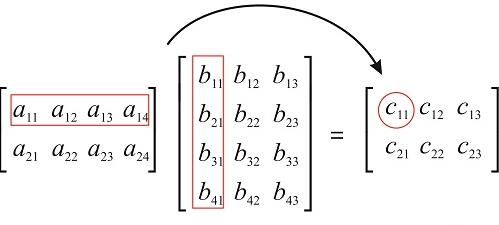
\includegraphics[width=0.5\linewidth]{matrix_chunk1} \end{center}

La entrada \(c_{22}\) de la matriz \(C=AB\) resultante es el producto
punto del renglón 2 de \(\mathbf{A}\) \(\mathbf{a}_{2\cdot}\) y la
columna 2 de \(\mathbf{B}\), \(\mathbf{b}_{\cdot 2}\).

\begin{center}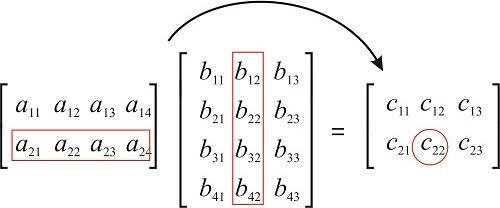
\includegraphics[width=0.5\linewidth]{matrix_chunk2} \end{center}

La multiplicación matricial se puede aplicar para los casos en que uno
de los elementos es un vector (interpretando a dicho vector como una
matriz de tamaño \(1\times n\) o \(m\times 1\)).

\hypertarget{ejemplo-2-1}{%
\subsubsection{Ejemplo 2}\label{ejemplo-2-1}}

\begin{enumerate}
\def\labelenumi{\alph{enumi})}
\tightlist
\item
  Sea \(A=\begin{pmatrix} 1 & -1 & 1 \end{pmatrix}\) y
  \(B=\begin{pmatrix} 7 \\ 0 \\ 5 \end{pmatrix}\). Determinar que
  productos son posibles \(A\cdot B\) y/o \(B\cdot A\).
\item
  Determinar el producto de las matrices
\end{enumerate}

\begin{equation*}
  \begin{array}{cccc}
   & \begin{bmatrix} 3 & -1 & 4 & 0  \end{bmatrix} &\cdot &  
     \begin{bmatrix} 1 \\-2 \\ 3\\ 1 \end{bmatrix}  \\  
  \end{array},
\end{equation*}

\begin{equation*}
  \begin{array}{cccc}
   & \begin{bmatrix} 
        1 & -1 & 0 & 2 \\
        0 &  1 & 3 & 4 \\
        2 &  0 &-1 & 3
      \end{bmatrix} &\cdot &  
     \begin{bmatrix} 2 \\-1 \\ 0\\ 3 \end{bmatrix}  \\  
  \end{array},
\end{equation*}

\hypertarget{respuesta}{%
\paragraph{\texorpdfstring{\emph{Respuesta}}{Respuesta}}\label{respuesta}}

a)\(A\) es una matriz \(1\times 4\) y \(B\) es una matriz \(4\times 1\).
Entonces, \(A\cdot B\) esta definido pues las columnas de \(A\) = los
renglones de \(B\) y el resultado será una matriz de tamaño
\(1\times 1\) es decir un escalar.

En este caso \(A\cdot B = 1\cdot 7 + (-1) \cdot 0 + 1\cdot 5\) = (12) =
12. Por otro lado \(B\cdot A\) también esta definido y el resultado será
una matriz de tamaño \(4\times 4\).

\begin{equation*}
  \begin{array}{cccc}
   & \begin{bmatrix} 
        7\cdot 1 & 7\cdot(-1) & 7\cdot 1  \\
        0\cdot 1 & 0\cdot(-1) & 0\cdot 1  \\
        5\cdot 1 & 5\cdot(-1) & 5\cdot 1 
      \end{bmatrix} & = & 
      \begin{bmatrix} 
        7 & -7 & 7  \\
        0 & 0  & 0  \\
        5 & -5 & 5 
      \end{bmatrix}
  \end{array} ,
\end{equation*}

\hypertarget{matrices-1}{%
\section{Matrices}\label{matrices-1}}

\hypertarget{propiedades-de-las-operaciones-on-matrices}{%
\subsection{Propiedades de las operaciones on
Matrices}\label{propiedades-de-las-operaciones-on-matrices}}

\small

1.- Para toda matriz \(A\) y \(\alpha,\beta\in \mathbb{R}\).

\begin{itemize}
\item
  \(1 \cdot \textbf{A}\) = \(\textbf{A} \cdot 1\) = \(\textbf{A}\).
\item
  \(0\cdot \mathbf{A}\) =\(\mathbf{A}\cdot 0\) = \(\mathbf{0}\).
\item
  \(\alpha \cdot (\beta\cdot A) = (\alpha \beta)\mathbf{A}\).
\end{itemize}

2.- Si \(A\), \(B\) y \(C\) tienen el mismo orden.

\begin{itemize}
\tightlist
\item
  \(\mathbf{A} + (\mathbf{B} + \mathbf{C}) = (\mathbf{A} + \mathbf{B}) + \mathbf{C}\).
\item
  \(\mathbf{A} + \mathbf{B} = \mathbf{B} + \mathbf{A}\).
\item
  \((\alpha+\beta)\cdot A = \alpha\cdot \mathbf{A} + \beta \cdot \mathbf{B}\).
\item
  \(\alpha \cdot (\mathbf{A}+ \mathbf{B}) = \alpha\cdot \mathbf{A} + \alpha \cdot \mathbf{B}\).
\item
  \(\mathbf{A}+\mathbf{0} = \mathbf{0}+\mathbf{A}=\mathbf{A}\)
\end{itemize}

\hypertarget{multiplicacion-de-matrices}{%
\subsection{Multiplicacion de
Matrices}\label{multiplicacion-de-matrices}}

\small

3.- Si \(A\), \(B\) y \(C\) tienen el orden adecuado.

\begin{enumerate}
\def\labelenumi{\alph{enumi})}
\tightlist
\item
  \((A+B)C = AC + BC\).
\item
  \(C(A+B) = CA + CB\).
\item
  \(A(BC) = (AB)C\).
\end{enumerate}

Para ver la \emph{asociatividad}, sea \(M=AB\) y \(N=BC\) queremos
verificar que \(AN = MC\). Por definición de la multiplicación de
matrices \[
\begin{array}{cc}
m_{ij} = & \sum_{k=1}^{n}a_{ik}b_{kj}. \\
n_{ij} = & \sum_{r=1}^{p}b_{ir}b_{rj}.
\end{array}
\] Entonces \[
\big( MC \big)_{ij}=\sum_{l=1}^{p}m_{il}c_{lj} = \sum_{l=1}^{p} \sum_{k=1}^n a_{ik}b_{kl}c_{lj} =  \sum_{k=1}^n a_{ik} \sum_{l=1}^{p}  b_{kj}c_{lj}
\] \[
=\sum_{k=1}^na_{ik}n_{kj}=(AN)_{ij}
\]

De la fórmula se deduce que el producto de varias matrices dispuestas en
un orden determinado no dependen de qué producto se hace primero.

\hypertarget{multiplicacion-de-matrices-1}{%
\section{Multiplicacion de
Matrices}\label{multiplicacion-de-matrices-1}}

\small

Por ejemplo, por asociatividad \[
((AB)C)D = (A(BC))D = A((BC)D)
\]

\hypertarget{potencias-de-matrices}{%
\subsection{Potencias de matrices}\label{potencias-de-matrices}}

Sea \(M\) una matriz \textbf{cuadrada} de orden \(n\), por definición

\begin{equation*}
M^{0}=Id(n)\,\,M^{1} = M\,\,  M^{2} = MM\,\, M^{3} = MMM.
\end{equation*}

En general \[
\begin{array}{cc}
M^{p}M^{q}= M^{p+q}\\
(M^{p})^{q} = M^{pq}
\end{array}
\]

\emph{Observación} : Las propiedades de productos notables no se
conserven.

\[
\begin{array}{cccc}
(A+B)^{2} & = & (A+B)(A+B) &= A^2 + AB + BA + B^2 \\
(A+B)(A-B) &= &A(A-B) + B(A-B)& = A^2 -AB + BA -B^2
\end{array}
\]

\hypertarget{matriz-transpuesta}{%
\subsection{Matriz transpuesta}\label{matriz-transpuesta}}

\small

Sea \(A=(a_{ij})\) una matriz de orden \(m\times n\), la matriz
transpuesta de \(A\), \(A^{T}\) es la matriz de orden \(n\times m\) tal
que \((A^T)_{ij}=A_{ji}\). \begin{equation*}
\begin{array}{ccccc}
A = & \begin{pmatrix} 3 & -2  \\ -4 & 3 \end{pmatrix} &\,\,\,\, & A^{T} = & \begin{pmatrix} 3 & -4  \\ -2 & 3 \end{pmatrix}  \\
\end{array}
\end{equation*}

\begin{equation*}
\begin{array}{ccccc}
A = & \begin{pmatrix} 3 & -1 & 0 \\ -2 & 1 & 1 \\ 2 & -1 & 4 \end{pmatrix} &\,\,\,\, & A^{T} = & \begin{pmatrix}  3 & -2 & 2 \\ -1 & 1 & -1 \\ 0 & 1 & 4  \end{pmatrix}  \\
\end{array}
\end{equation*}

\begin{equation*}
\begin{array}{ccccc}
A = & \begin{pmatrix} -1 & 3 & 0 \\ -2 & 1 & 1 \\ 3 & 0 & -2 \\ 4 & 1 & 2 \end{pmatrix} &\,\,\,\, & A^{T} = & \begin{pmatrix}  -1 & -2 & 3 & 4 \\ 3 & 1 & 0 &  1 \\ 0 & 1 & -2 & 2  \end{pmatrix}  \\
\end{array}
\end{equation*}

\hypertarget{propiedades-de-la-matriz-transpuesta}{%
\subsection{Propiedades de la matriz
transpuesta}\label{propiedades-de-la-matriz-transpuesta}}

\begin{enumerate}
\def\labelenumi{\arabic{enumi})}
\tightlist
\item
  \((\alpha A + \beta B)^{T} = \alpha A^{T} + \beta B^{T}\).
\item
  \((AB)^{T} = B^{T}A^{T}\).
\item
  \(\big(A^{T}\big)^{T}=A\)
\end{enumerate}

La primer propiedad es fácil de verificar.

Si \(a_{ij}\) y \(b_{ij}\) son las entradas de las matrices \(A\) y
\(B\) respectivamente, entonces las entradas de \(A^{T}\) y \(B^{T}\)
son \(a_{ji}\) y \(b_{ji}\) por lo que

\[
(A^{T} + B^{T})_{ij} = (a_{ji}+b_{ji})\quad\quad\mbox{ para }j=1,2,\ldots,m,\,\,i=1,2,\ldots,n
\] Pero el último término corresponde con las entradas de \((A+B)^{T}\).

La segunda propiedad se cumple por la siguiente razón \begin{equation*}
  [(AB)^T]_{ij} = \sum_{k=1}^m a_{jk}b_{ki} = \sum_{k=1}^m b^T_{ik} a^T_{kj} = [B^TA^T]_{ij}
\end{equation*}

\hypertarget{definiciuxf3n-2}{%
\subsection{Definición:}\label{definiciuxf3n-2}}

Si \(\mathbf{A}\) es una matriz cuadrada de orden \(n\) y
\(\mathbf{A}=\mathbf{A}^{T}\) decimos que \(\mathbf{A}\) es una matriz
\textbf{simétrica}. Si \(\mathbf{A}=-\mathbf{A}^{T}\) decimos que es
\textbf{antisimétrica}.

\hypertarget{matriz-conjugada}{%
\subsection{Matriz conjugada}\label{matriz-conjugada}}

\small

Sea \(A=(a_{ij})\) una matriz de orden \(m\times n\) de números
complejos, la matriz \textbf{conjugada} de \(A\), \(\bar{A}\) es la
matriz de orden \(m\times n\) tal que \((\bar{A})_{ij}=\bar{a_{ij}}\).

Sea \(A=(a_{ij})\) una matriz de orden \(m\times n\) de números
complejos, la matriz \textbf{transpuesta} \textbf{conjugada} de \(A\),
\(A^{*}\) es la matriz de orden \(n\times m\) tal que
\((A)_{ij}=(\bar{A})_{ji}\). Es decir, la adjunta de \(A\) se obtiene al
\emph{conjugar} y \emph{transponer} \(A\).

\begin{equation*}
\begin{array}{ccccc}
A = & \begin{pmatrix} -i & 2 + 3i  \\ -4i & 5+2i \end{pmatrix} &\,\,\,\, & A^{*} = & \begin{pmatrix} i & 4i  \\ 2-3i & 5-2i \end{pmatrix}  \\
\end{array}
\end{equation*}

Si \(\mathbf{A}\) es una matriz cuadrada y \(A\) es igual a su adjunta,
entonces se dice que \(\mathbf{A}\) es una matriz \textbf{hermitiana} o
\textbf{simétrica} \textbf{según} \textbf{Hermite}.

\hypertarget{matriz-inversa}{%
\subsection{Matriz Inversa}\label{matriz-inversa}}

\small

Si \(\mathbf{A}\) es una matriz cuadrada de orden \(n\), se dice que
\(X\) es la matriz \textbf{inversa} de \(A\) si \[
A\cdot X = X\cdot A = \mathbf{Id}
\]

Si dicha matriz existe decimos que \(A\) es \textbf{invertible}. La
matriz inversa de \(A\) se escribe como \(A^{-1}\).

\hypertarget{ejemplo-3}{%
\subsection{Ejemplo}\label{ejemplo-3}}

Calcular la matriz inversa de

\[
A =  \begin{pmatrix} 1 & 1 & 1  \\ 1 & 2 & 2 \\ 1 & 2 & 3 \end{pmatrix}
\]

\[
B =  \begin{pmatrix} 1 & 2 \\ -2 & 4  \end{pmatrix}
\]

Para calcular la inversa, se requiere resolver \(n\) sistemas de
ecuaciones, cada uno con
\(\vec{b}=\mathbf{e}_i=\begin{pmatrix} 0, \ldots,0,1,0,\ldots,0 \end{pmatrix}\)

Para evitar repetir la matriz aumentada conservamos \emph{cada}
\emph{término} \emph{independiente} en una matriz ampliada \[
  \begin{bmatrix}
        a_{11}   & \cdots   & a_{1n}   &\bigm| & 1       & 0      & \cdots  & 0 \\
        a_{21}   & \cdots   & a_{2n}   &\bigm| & 0       & 1      & \cdots  &  0\\
    \vdots       & \vdots   & \vdots   &\bigm| & \vdots  & \ddots & \cdots  & 0 \\
      a_{n1}  & \cdots      & a_{nn}   &\bigm| & 0       & 0      & \cdots  & 1
  \end{bmatrix}
\] Y procedemos a aplicar operaciones elementales, en vez de obtener una
matriz triangular superior, y aplicar sustitución hacia atrás, aplicamos
operaciones elementales para obtener una \textbf{matriz}
\textbf{identidad}.

\begin{equation*}
  \begin{bmatrix}
        1   & 2 &\bigm| & 1       & 0     \\
        -2  & 4  &\bigm| & 0       & 1     
  \end{bmatrix} 
  \xrightarrow{2E_1+E_2\rightarrow E_2}
  \begin{bmatrix}
        1   & 2  &\bigm| & 1       & 0     \\
        0   & 8  &\bigm| & 2       & 1     \\
  \end{bmatrix} 
  \xrightarrow{1/8E_2\rightarrow E_2}
\end{equation*}

\[
  \begin{bmatrix}
        1   & 2  &\bigm| & 1         & 0     \\
        0   & 1  &\bigm| & 1/4       & 1/8     \\
  \end{bmatrix} 
  \xrightarrow{-2E_2+E_1\rightarrow E_1}
  \begin{bmatrix}
        1   & 0  &\bigm| & 1/2         & -1/4     \\
        0   & 1  &\bigm| & 1/4       & 1/8     \\
  \end{bmatrix} 
\]

A diferencia de eliminación gaussiana, el algoritmo termina cuando
podemos encontrar una diagonal en la matriz izquierda. \textbf{Si}
\textbf{esto} \textbf{es} \textbf{posible}, la matriz del lado derecho
será la inversa.

Pues son las soluciones a los sistemas

\begin{equation*}
  \begin{matrix}
           x  & +2 y  & = 1  \\
           -2x & +4 y   & = 0   
  \end{matrix} \quad \mbox{ y }\quad
  \begin{matrix}
           x  & +2 y  & = 0  \\
           -2x & +4 y   & = 1   
  \end{matrix}
\end{equation*}

\hypertarget{aplicar-eliminaciuxf3n-gaussiana-para-invertir-a.}{%
\subsubsection{\texorpdfstring{Aplicar eliminación gaussiana para
invertir
\(A\).}{Aplicar eliminación gaussiana para invertir A.}}\label{aplicar-eliminaciuxf3n-gaussiana-para-invertir-a.}}

\hypertarget{teorema}{%
\subsection{Teorema}\label{teorema}}

Si \(A\) es invertible, para \textbf{cualquier}
\(\mathbf{b}\in\mathbb{R}^{n}\), el sistema de ecuaciones: \(Ax =b\) con
: \begin{equation*}
A =   \left[
  \begin{matrix}
     a_{11}   & \cdots   & a_{1n} \\
    \vdots    &          & \vdots \\
      a_{n1}  & \cdots        & a_{nn}
  \end{matrix}
  \right]
\end{equation*}

\begin{equation*}
  \mathbf{x} =
    
  \begin{pmatrix}
     x_1 \\
     x_2 \\
     \vdots \\
     x_n
  \end{pmatrix}
     \hspace{.2cm}
   \mbox{  y  }
   \hspace{.2cm}  
   \mathbf{b} =
      \begin{pmatrix}
       b_1 \\
       b_2 \\
       \vdots \\
       b_n
    \end{pmatrix}
\end{equation*}

tiene \textbf{solución} \textbf{única} y es igual a

\begin{equation*} \label{sistema}
  x = \mathbf{A}^{-1}\mathbf{b}
\end{equation*}

Calcular la inversa para solucionar un sistema de ecuaciones es poco
eficiente. Sin embargo, es útil para solucionar una \emph{familia}
\emph{de} \emph{sistemas} \emph{de} \emph{ecuaciones}.

\hypertarget{ejemplo-4}{%
\subsection{Ejemplo}\label{ejemplo-4}}

\begin{enumerate}
\def\labelenumi{\arabic{enumi}.}
\item
  verificar que la siguiente matriz es la inversa de \(A\)
\item
  Calcular la inversa de la matriz \(A\)
\end{enumerate}

\begin{equation*}
  A = \begin{pmatrix}
          1 & 1 & 1 \\
          1 & 2 & 2 \\
          1 & 2 & 3 
      \end{pmatrix}
\end{equation*}

\begin{enumerate}
\def\labelenumi{\arabic{enumi}.}
\tightlist
\item
  Calcular la matriz inversa de
\end{enumerate}

\begin{equation*}
 \begin{bmatrix} 3 & -5 & 1   \\  
                 0 & 1  & -1  \\ 
                 3 & 5  & 7   
 \end{bmatrix}  
\end{equation*}

\hypertarget{ejercicios-1}{%
\section{Ejercicios}\label{ejercicios-1}}

\begin{equation*}
\begin{array}{ccccc}
A = & \begin{pmatrix} 1 & -1 & 2  \\ 0 & 3 & 4 \end{pmatrix} &\,\,\,\, & 
B = & \begin{pmatrix} 4 & 0 & -3  \\ -1 & -2 & 3 \end{pmatrix}  \\
C = & \begin{pmatrix} 2 & -3 & 0 & 1  \\ 5 & -1 & -4 & 2 \\ -1 & 0 & 0 & 3 \end{pmatrix} &\,\,\,\, &
D = & \begin{pmatrix}  2  \\ -1 \\ 3 \end{pmatrix}  \\
\end{array}
\end{equation*}

\begin{itemize}
\item
  Calcular \(3A - 4B\), \(AC\), \(BC\), \(AD\), \(BD\), \(CD\)
\item
  Encontrar \(A^{T}\) y \(A^{T}B\) y \(A^{T}C\).
\end{itemize}

Usando la definición de inversa, calcular \(A^{-1}\) si
\(A=\begin{pmatrix} 1 & 1 & 1 \\ 0 & 1 & 2 \\ 1 & 2 & 4 \end{pmatrix}\)

Encuentra \(x,y,z\) tal que \(A\) es simétrica \[
A = \begin{pmatrix} 2 & x & 3  \\ 4 & 5 & y\\ z & 1 & 7 \end{pmatrix}
\]

Encuentra \(x,y,z\) tal que \(A\) es hermitiana \[
A = \begin{pmatrix} 3 & x+2i & yi  \\ 3-2i & 0 & 1+iz\\ yi & 1-xi & -1 \end{pmatrix}
\]

\hypertarget{propiedades-de-la-matriz-inversa}{%
\subsection{Propiedades de la matriz
inversa}\label{propiedades-de-la-matriz-inversa}}

\hypertarget{definiciuxf3n-3}{%
\subsubsection{Definición}\label{definiciuxf3n-3}}

Una matriz es singular si existe \(\mathbf{x}\ne \mathbf{0}\) que es
solución al sistema

\begin{equation}
\mathbf{A}\cdot \mathbf{x} = \mathbf{0}
\end{equation}

Una matriz es \textbf{no} \textbf{singular} si: para todo
\(x\in\mathbb{R}^{n}\), si \(\mathbf{x}\ne \mathbf{0}\) entonces
\(\mathbf{A}\mathbf{x}\ne \mathbf{0}\). Es decir una matriz es no
singular si el conjunto solución del sistema
\(\mathbf{A}\mathbf{x}=\mathbf{0}\) es sólo el conjunto
\(\{\mathbf{0}\}\).

De los resultados previos, sabemos que si \(A\) es invertible entonces
\(\mathbf{A}\vec{\mathbf{x}} = \vec{\mathbf{0}}\) tiene una única
solución
\(\vec{\mathbf{x}} = \mathbf{A}^{-1}\vec{\mathbf{0}}=\vec{\mathbf{0}}\).

Esto significa

\begin{itemize}
\tightlist
\item
  Si \(A\) es invertible, entonces \(A\) es \textbf{no}
  \textbf{singular}.
\end{itemize}

Propiedades

\begin{enumerate}
\def\labelenumi{\arabic{enumi})}
\item
  Si \(A\) es invertible, y tanto \(X_1\) como \(X_2\) cumple con
  \(X_1\cdot A=\mathbf{I}_n=A\cdot X_1\) y
  \(X_2\cdot A=\mathbf{I}_n=A\cdot X_2\) entonces \(X_1=X_2=A^{-1}\). Es
  decir, la inversa es única.
\item
  Si \(A\) es invertible, entonces \(A^{-1}\) también es invertible y \[
  \Big(A^{-1}\Big)^{-1} = A 
  \]
\item
  Si \(A\) y \(B\) son matrices de orden \(n\) e invertibles entonces
  \(AB\) es invertible. Además \begin{equation}
   (AB)^{-1} = B^{-1} A^{-1}
  \end{equation}
\item
  Si \(A_1\), \(A_2,\ldots,A_n\) son matrices invertibles de orden
  \(n\), entonces el producto \(A_1\cdot A_2\cdot\ldots\cdot A_n\) es
  invertible.
\end{enumerate}

\begin{equation}
 (A_1A_2\ldots A_n)^{-1} = A_n^{-1}\cdot A_{n-1}^{-1}\cdots A_1^{-1}
\end{equation}

\begin{enumerate}
\def\labelenumi{\arabic{enumi})}
\setcounter{enumi}{4}
\tightlist
\item
  Si \(A\in\mathcal{M}^{n}(\mathbb{R})\) una matriz de orden \(n\)
  entonces \(A^{T}\) también es invertible y \begin{equation}
  \big(A^{T}\big)^{-1} = \big(A^{-1}\big)^{T}
  \end{equation}
\end{enumerate}

Explicación

\begin{enumerate}
\def\labelenumi{\arabic{enumi})}
\item
  Si \(X_1\) y \(X_2\) cumplen con \(X_1A = \mathbf{I}_n=X_2A\)
  entonces, \[
  X_1 = X_1\cdot \mathbf{I}_n = X_1\cdot(A\cdot X_2) = (X_1\cdot A)\cdot X_2 = \mathbf{I}_n\cdot X_2 = X_2 
  \] Esto también implica que si \(X_1\) es una matriz que es una
  inversa por la izquierda(por la derecha) entonces también es una
  inversa por la derecha(por la izquierda) y por tanto es la inversa de
  \(A\).
\item
  Si \(A\) es invertible entonces \(A\cdot A^{-1} = \mathbf{I}_n\) pero
  entonces \(A^{-1}\) también es invertible y la inversa de \(A^{-1}\)
  es \(A\). Dicho de otra forma
\end{enumerate}

\begin{equation}
 \big( A^{-1} \big)^{-1}
\end{equation}

\begin{enumerate}
\def\labelenumi{\arabic{enumi})}
\setcounter{enumi}{2}
\tightlist
\item
  Suponga que \(A\) y \(B\) son invertibles entonces, sea
  \(X=B^{-1}A^{-1}\). Entonces \[
  AB\cdot X=AB\cdot B^{-1}A^{-1} = A\mathbf{I}_n\cdot A^{-1} = \mathbf{I}_n 
  \]
\end{enumerate}

De manera similar, se tiene 4).

\hypertarget{observaciuxf3n-1}{%
\subsubsection{Observación}\label{observaciuxf3n-1}}

Si \(\mathbf{A}\in\mathcal{M}^{n}(\mathbb{R})\) es invertible entonces,
para cualquier \(\mathbf{b}\in\mathbb{R}^{n}\) \[
\mathbf{A}\vec{\mathbf{x}} = \vec{\mathbf{b}}
\] Tiene una solución única. Y además
\(\vec{\mathbf{x}} = \mathbf{A}^{-1}\vec{\mathbf{b}}\).

En particular, el sistema homogéneo también tiene una solución única, la
trivial.

Usando la última observación, resolver los siguientes sistemas

\begin{equation*}
  \begin{matrix}
           x   & +3 y  &+2z  & = b_1  \\
           15x & +2 y &  & = b_2   \\
           4x & +2 y &  +z & = b_3
  \end{matrix}
\end{equation*}

Con \(\begin{pmatrix}2 \\ 2 \\1 \end{pmatrix}\) y
\(\begin{pmatrix}1 \\ -2 \\0 \end{pmatrix}\)

\hypertarget{forma-escalonada-y-forma-escalonada-reducida}{%
\subsection{Forma escalonada y forma escalonada
reducida}\label{forma-escalonada-y-forma-escalonada-reducida}}

Estudiamos brevemente el caso en donde hay más incógnitas que
ecuaciones, es decir, sistemas \(m\times n\) con \(m<n\).

\hypertarget{ejemplo-1-2}{%
\subsubsection{Ejemplo 1}\label{ejemplo-1-2}}

Resolver el sistema definido por la matriz extendida

\begin{equation*}
 \begin{array}{cc}
  [\mathbf{A}| \mathbf{b}] & = \begin{pmatrix}
                                  1   &   3 &   3  & 2 &\biggm| & 1  \\
                                  2   &   6 &   9  & 5 &\biggm| & 2   \\
                                 -1   &  -3 &   3  & 0 &\biggm| & 0
                                \end{pmatrix}
 \end{array}
\end{equation*}

Aplicando eliminación gaussiana obtenemos

\[
\begin{pmatrix}
                                  1   &   3 &   3  & 2 &\biggm| & 1  \\
                                  0   &   0 &   3  & 1 &\biggm| & 0   \\
                                  0   &   0 &   0  & 0 &\biggm| & 0
                                \end{pmatrix}
\]

El sistema es \textbf{consistente}. En este caso la matriz tiene forma
triangular superior, pero los pivotes no están necesariamente :en\_
\emph{la} \emph{diagonal} sino a la derecha de la diagonal. Decimos que
la matriz tiene una forma \textbf{escalonada}.

\hypertarget{definiciuxf3n-4}{%
\subsubsection{Definición}\label{definiciuxf3n-4}}

Una matriz está en forma escalonada si

\begin{enumerate}
\def\labelenumi{\arabic{enumi})}
\item
  Primero vienen las filas distintas de cero (sino se intercambian) y
  para cada una de las filas (distinas de cero) los pivotes son las
  \emph{primeras} \emph{entradas} \emph{distintas} \emph{de} \emph{cero}
  en esas filas.
\item
  Debajo de cada pivote hay una columna de ceros, obtenida de la
  eliminación.
\item
  Cada pivote está a la derecha del pivote de la fila anterior.
\end{enumerate}

En ocasiones el método de eliminación gaussiana no produce una forma
triangular y no es posible tomar como pivote la diagonal ``inmediata''.

\hypertarget{ejemplo-2-2}{%
\subsection{Ejemplo 2}\label{ejemplo-2-2}}

Aplicar eliminación gaussiana al siguiente sistema

\begin{equation*}
  \begin{matrix}
           x_1  & +2 x_2 & +x_3 & +3x_4 & +3x_5& = 5  \\
           2x_1 & +4 x_2 &      & +4x_4 & +4x_5& = 6  \\
           x_1  & +2 x_2 & +3x_3 & +5x_4 & +5x_5& = 9  \\
           2x_1  & +4 x_2 &      & +4x_4 & +7x_5& = 9  \\
  \end{matrix}
\end{equation*}

(Ver notas)

\hypertarget{algoritmo-modificado-de-eliminaciuxf3n-gaussiana}{%
\subsection{Algoritmo modificado de eliminación
gaussiana}\label{algoritmo-modificado-de-eliminaciuxf3n-gaussiana}}

Suponga que \(U\) es la matriz aumentada asociada al sistema de
ecuaciones, después de la \(i-\)esima iteración.

\begin{itemize}
\item
  Moverse de izquierda a derecha en \(U\), localizar la primer columna
  que contiene la entrada no nula en la \(i-\)esima fila o posterior,
  digamos en la entrada \((i,j)\).
\item
  La nueva posición pivotal será la entrada \((i,j)\).
\item
  Aplicar la eliminación a partir de dicho elemento.
\item
  Si todas las filas posteriores al proceso de eliminación son nulas, el
  proceso de eliminación gaussiana concluye.
\end{itemize}

Todo sistema de ecuaciones de tamaño \(m\times n\) con más incógnitas
que ecuaciones (\(m<n\)) tendrá una matriz escalonada en forma
rectangular. Al tener más variables que incógnitas, habrá \(n-m\)
parámetros libres.

\hypertarget{teorema-1}{%
\subsection{Teorema}\label{teorema-1}}

\emph{Todo} \emph{sistema} \emph{de} \emph{ecuaciones} \emph{de}
\emph{tamaño} \(m\times n\) \emph{con} \(m<n\) \emph{o} \emph{bien}
\emph{es} \emph{inconsistente} \emph{o} \emph{tiene} \emph{una}
\emph{infinidad} \emph{de} \emph{soluciones}

\hypertarget{ejemplo-3-1}{%
\subsection{Ejemplo 3}\label{ejemplo-3-1}}

Resolver el siguiente sistema

\begin{equation*}
  \begin{matrix}
        2x   &  +2y & +2z & = 5  \\
         x   &  +2y & -z  & = 4
  \end{matrix}
\end{equation*}

\begin{equation*}
 \begin{array}{ccccc}
   U & = \begin{pmatrix}
                                  2   &   2 &   2  & 5   \\
                                  1   &   2 &   -1 & 4    
                                \end{pmatrix} & \quad\rightarrow \quad
    & (R_1 \leftrightarrow R_2)  
        &= \begin{pmatrix}
                                  1   &   2 &   -1  & 4   \\
                                  2   &   2 &    2  & 5   
                                \end{pmatrix}
 \end{array}
\end{equation*}

\(-2R_1 + R2\) \begin{equation*}
 \begin{array}{ccccc}
   \rightarrow & = \begin{pmatrix}
                           1   &   2 &   -1  & 4   \\
                           0   &   -2 &   4  & -3    
                                \end{pmatrix} & \quad\rightarrow \quad
    & (R_2/2 \leftrightarrow R_2)  
        &= \begin{pmatrix}
                                  1   &   2 &   -1  & 4   \\
                                  0   &   1 &    -2  & \frac{3}{2}   
                                \end{pmatrix}
 \end{array}
\end{equation*}

El resultado del algoritmo de eliminación gaussiana es una matriz con
``ceros'', si el sistema tiene solución única, el resultado final es una
matriz triangular superior. En otros casos es una matriz que tiene
renglones en \(0'\)s.

\#\#Matriz escalonada reducida

\hypertarget{definiciuxf3n-5}{%
\subsubsection{Definición}\label{definiciuxf3n-5}}

Una matriz esta en su \textbf{forma} (\textbf{normal})
\textbf{escalonada} \textbf{reducida} si las siguientes condiciones se
cumplen

\begin{enumerate}
\def\labelenumi{\arabic{enumi})}
\item
  Los renglones nulos están debajo de los renglones no nulos.
\item
  La primer entrada o pivote, para cada renglón no nulo es \(1\),
\item
  La columna que contiene el primer elemento no nulo, para un renglón,
  tiene \(0'\)s en las otras filas.
\item
  El pivote de una fila debe estar más a la derecha que los pivotes de
  filas previas
\end{enumerate}

\hypertarget{ejemplo-4-1}{%
\subsubsection{Ejemplo 4}\label{ejemplo-4-1}}

La primera matriz está en su forma escalonada reducida

\begin{equation*}
 \begin{array}{ccccc}
   U & = \begin{pmatrix}
                                  1   &   2 &   0  & 0 & -3 &  1  & 0   \\
                                  0   &   0 &   1  & 0 &  4 & -1  & 0   \\
                                  0   &   0 &   0  & 1 &  3 & -2  & 0   \\
                                  0   &   0 &   0  & 0 &  0 &  0  & 1   \\
                                  0   &   0 &   0  & 0 &  0 &  0  & 0   
                                \end{pmatrix} & \quad\quad\quad
    & U_2 &= \begin{pmatrix}
                                  1   &   0 &   0  & 0 &  1    \\
                                  0   &   0 &   1  & 0 &  2   \\
                                  0   &   1 &   0  & 1 &  1    \\
                                  0   &   0 &   0  & 0 &  0    \\
                                  0   &   0 &   0  & 0 &  0 
                                \end{pmatrix}
 \end{array}
\end{equation*}

La matriz \(U_2\) no está en su forma escalonada reducida, pues los
pivotes del tercer renglón no se encuentra a la derecha del pivote del
segundo renglón

\hypertarget{ejemplo-5}{%
\subsubsection{Ejemplo 5}\label{ejemplo-5}}

Resolver el sistema de ecuaciones usando eliminación gaussiana. Obtener
su forma escalonada, resolver la ecuación. Obtener su forma escalonada
reducida y resolver la ecuación resultante

\begin{equation*}
  \begin{matrix}
         x   &  -y & +z & = 7  \\
         2x   &  +y & +z  & = 5
  \end{matrix}
\end{equation*}

Aplicando operaciones elementales obtenemos

\begin{equation*}
 \begin{array}{ccccc}
   \mathbf{A}|\mathbf{b} & = \begin{pmatrix}
                                  1   & -1 &   1  &|& 7   \\
                                  2   &  2 &   1  &|& 5    
                                \end{pmatrix} & \quad\rightarrow \quad
    & (-2R_1 + R_2 \leftrightarrow R_2)  
        &= \begin{pmatrix}
                                  1   & -1 &  1  &|& 7   \\
                                  0   &  3 & -1  &|& -9   
                                \end{pmatrix}
 \end{array}
\end{equation*} Una forma escalonada es la matriz anterior

\[
\begin{array}{ccc}
U &= & \begin{pmatrix} 
                   1   & -1 &  1  &\big|& 7   \\
                  0   &  3 & -1  &\big|& -9   
        \end{pmatrix}
\end{array} 
  \quad\quad\mbox{ otra forma es }\quad\quad
\begin{array}{ccc}
U' &= & \begin{pmatrix} 
                   1   & -1 &  1  &\big|& 7   \\
                  0   &  1 & -\frac{1}{3}  &\big|& -3   
        \end{pmatrix}
\end{array}
\] que se obtiene dividiendo el segundo renglón entre \(3\). Sin
embargo, ninguna de las anteriores es la forma escalonada
\emph{reducida}. Para obtener la forma escalonada reducida, debemos
tener entradas nulas \emph{arriba} y \emph{abajo} de los pivotes y las
primeras columnas no nulas en las ecuaciones pivotales deben ser 1. Es
decir, para obtener la forma escalonada reducida en la segunda matriz de
éste ejemplo hay que eliminar la entrada del primer renglón arriba del
segundo pivote (-1). \begin{equation*}
 \begin{array}{ccccc}
   \mathbf{A}|\mathbf{b} & = \begin{pmatrix}
                                   1   & -1 &  1            &\big|& 7   \\
                                   0   &  1 & -\frac{1}{3}  &\big|& -3   
                                \end{pmatrix} & \quad\rightarrow \quad
    & (R_2 + R_1 \leftrightarrow R_1)  
        &= \begin{pmatrix}
                                  1   &  0 &  \frac{2}{3}  &|& 7   \\
                                  0   &  1 & -\frac{1}{3}  &|& -3´    
                                \end{pmatrix}
 \end{array}
\end{equation*}

\hypertarget{ejercicios-2}{%
\section{Ejercicios}\label{ejercicios-2}}

\small

Obtener la expresión matricial de la matriz escalonada reducida del
sistemas de ecuaciones lineales en los ejemplos de la clase.

Para el siguiente sistema

\begin{equation*}
  \begin{matrix}
      x_1   & -2 x_2  & +2 x_3  & = 0  \\
      2 x_1 &  - x_2  & +5 x_3  & = 0 \\
      x_1   &  + x_2  & +4 x_3  & = 0 
  \end{matrix}
\end{equation*}

Encontrar la \textbf{matriz} \textbf{escalonada} \textbf{reducida} del
sistema

La matriz del sistema y la matriz extendida asociada
\([\mathbf{A}|\mathbf{b}]\) al sistema es \(\mathbf{A}= ?\) y
\([\mathbf{A}|b]\) \begin{equation*}
  \begin{matrix}
            &  2 x_2 &+ 3 x_3  & = 8  \\
     2 x_1  & + 3x_2 & +  x_3  & = 5   \\
      x_1   &  -x_2  &  -2 x_3  & =-5
  \end{matrix}
\end{equation*} \([\mathbf{A} | \mathbf{b}] =?\)

\hypertarget{importancia-de-la-matriz-escalonada-reducida.}{%
\subsection{Importancia de la matriz escalonada
reducida.}\label{importancia-de-la-matriz-escalonada-reducida.}}

\hypertarget{teorema-2}{%
\subsubsection{Teorema}\label{teorema-2}}

Suponga que tenemos un sistema de ecuaciones lineales \(n\times m\),
homogéneo, con \(n<m\), es decir,

\begin{equation}
  \begin{matrix}
     a_{11} x_1 & +a_{12} x_2 + & \cdots   & +a_{1m} x_m  &= 0  \\
     a_{21} x_1 & +a_{22} x_2 + & \cdots   & +a_{2m} x_m  &= 0  \\
    \vdots    & \vdots  & \vdots   & \vdots \\
     a_{n1} x_1 & +a_{n2} x_2 + & \cdots   & +a_{nm} x_m  &= 0
  \end{matrix}
\end{equation} entonces el sistema de ecuaciones lineales tiene una
\emph{infinidad} \emph{de} \emph{soluciones}.

Suponga que tenemos un sistema de ecuaciones lineales homogéneo
\(n\times m\) y que la matriz asociada al sistema es la \textbf{matriz}
\textbf{escalonada} \textbf{reducida}. \[
\mathbf{U}_{r}\vec{x} = \vec{0}
\] como \(\mathbf{U}_r\) la matriz escalonada, suponga que se tienen
\(r\leq n\) ecuaciones no nulas, es decir, \(r\) renglones no nulos.
Suponga que son las filas \(i=1,2\ldots,r\) filas y suponga que los
pivotes están en las columnas \(i_1,i_2,\ldots,i_r\), esto significa que
la incógnita \(x_{i_k}\) aparece solamente 1 vez, con coeficiente 1 en
la ecuación \(k\), y \(u_1,u_2,\ldots,u_{m-r}\) son las otras variables
del sistema, es decir,
\(u_1,u_2,\ldots, u_{m-r} \notin\{x_{i_1},x_{i_2},\ldots,x_{i_r}\}\)

por lo que las ecuaciones del sistema \(R\vec{x}=\vec{0}\) se escriben
como \begin{equation}
  \begin{matrix}
      x_{i_1}         & +c_{11} u_1 &  + \cdots +     & c_{1,m-r} u_{m-r}  &= 0  \\
      \,\,x_{i_2}     & +c_{21} u_1 &  + \cdots +     & c_{2,m-r} u_{m-r}  &= 0  \\
    \vdots            & \vdots      &  \vdots        & \vdots & \vdots \\
     \,\,\,\,x_{i_r}  & +c_{r1} u_1 &  + \cdots  & +c_{r,m-r} u_{m-r}  &= 0
  \end{matrix}
\end{equation}

Por lo que tenemos variables \emph{básicas}
\(x_{i_1},x_{i_2},\ldots,x_{i_r}\) que dependen de los valores dados a
\(u_1,u_2,\ldots,u_{m-r}\). Es decir, la solución al sistema de
ecuaciones \(n\times m\) existe y no es única.

\hypertarget{teorema-2-1}{%
\subsubsection{Teorema 2}\label{teorema-2-1}}

Si \(A\) es una mtriz \(n\times n\) y \(U_r\) es su matriz escalonada
reducida entonces \(U_r=\mathbf{I}_n\) si y sólo si
\(\mathbf{A}\vec{x}=\vec{\mathbf{0}}\) tiene una única solución.

\emph{Demostración}:

Si \(\mathbf{U}_r=\mathbf{I}_n\) entonces
\(\mathbf{A}\vec{x}=\vec{\mathbf{0}}\) y
\(\mathbf{I}_n\vec{x}=\vec{\mathbf{0}}\) tienen las mismas soluciones,
es decir la solución trivial. Ahora, suponga que el sistema tiene una
única solución y sea \(R\) la matriz escalonada reducida y \(r\) el
número de renglones no nulos, entonces \(r\leq n\), no es posible que
\(r < n\) por que entonces, por el teorema anterior, tendríamos más de
una solución, luego \(r=n\), pero como \$r=\# \$de pivotes en
\(\mathbf{U}_r\) entonces \(\mathbf{U}'_R=\mathbf{I}_n\)

Para el sistema homogéneo \[
  \mathbf{A}\vec{x} = \vec{\mathbf{0}}
  \] o bien el sistema tiene solución única
(\(\vec{x}=\vec{\mathbf{0}}\)) o bien tiene una infinidad de soluciones.

\hypertarget{matrices-elementales}{%
\section{Matrices elementales}\label{matrices-elementales}}

\small

\hypertarget{definiciuxf3n-de-las-matrices-elemental.}{%
\subsection{Definición de las matrices
elemental.}\label{definiciuxf3n-de-las-matrices-elemental.}}

Una \textbf{matriz} se dice ser \textbf{elemental} de orden \(n\) es una
matriz que se puede obtener de la matriz identidad \(\mathbf{I}_n\) por
medio de una sóla operacion elemental en sus filas.\\
A la operación elemental de intercambio de renglones se le asociará las
siguientes matrices

\hypertarget{intercambio-de-renglones}{%
\subsubsection{Intercambio de
renglones:}\label{intercambio-de-renglones}}

Considere a la matriz \(\mathbf{I}_n\), si le aplicamos la operación
elemental de intercambio de renglones \(i\leftrightarrow j\) obtenemos
la matriz que tiene como entrada
\(a_{ii}=0,\,\, a_{ij}=1,\,\, a_{jj}=0,\,\, a_{ji}=1\)

\begin{equation*}
\begin{array}{ccccc}
\mathbf{I}_n = &  \begin{bmatrix} 
                   1      & 0     & \ldots  & 0     & \cdots& 0      & 0       & 0      \\ 
                   0      & 1     & \ldots  & 0     & \cdots& 0      & 0       & 0      \\
                \vdots    & \vdots& \vdots  & \vdots& \vdots& \vdots & \vdots  & \vdots \\
                   0      &  0    & \ldots  & 1     & \cdots& 0      & 0       & 0      \\
                \vdots    & \vdots& \vdots  & \vdots& \vdots& \vdots& \vdots  & \vdots \\
                   0      &  0    & \ldots  & 0     & \cdots& 1      & 0       & 0      \\
                \vdots    & \vdots& \vdots  & \vdots& \vdots& \vdots & \vdots  & \vdots \\   
                  0       &  0    & \ldots  & 0     & \ldots& \ldots & 0      & 1
  \end{bmatrix}
 & \xrightarrow{ E_i\leftrightarrow E_j}
 &  \begin{bmatrix} 
     1      & 0     & \ldots  & 0     & \cdots  & 0      & 0       & 0      \\ 
     0      & 1     & \ldots  & 0     & \cdots  & 0      & 0       & 0      \\
  \vdots    & \vdots& \vdots  & \vdots& \vdots  & \vdots & \vdots  & \vdots \\
     0      &  0    & \ldots  & 0     & \cdots  & 1      & 0       & 0      \\
    \vdots  & \vdots& \vdots  & \vdots& \vdots  & \vdots & \vdots  & 0      \\
     0      &  0    & \ldots  & 1     & \cdots  & 0      & 0       & 0      \\
     \vdots & \vdots& \vdots  & \vdots& \vdots  & \vdots & \vdots  & \vdots \\
     0      &  0    & \ldots  & 0     & \cdots  & 0      & 0       & 1
  \end{bmatrix}
\end{array}
\end{equation*} El primer tipo de matrices elementales son las matrices
\(P_{ij}\)

\begin{equation*}
\begin{array}{cr}
P_{ij} = &  \begin{bmatrix} 
               1      & 0     & \ldots  & 0     & \cdots  & 0      & 0       & 0      \\ 
               0      & 1     & \ldots  & 0     & \cdots  & 0      & 0       & 0      \\
            \vdots    & \vdots& \vdots  & \vdots& \vdots  & \vdots & \vdots  & \vdots \\
               0      &  0    & \ldots  & 0     & \cdots  & 1      & 0       & 0      \\
             \vdots   & \vdots& \vdots  & \vdots& \vdots  & \vdots & \vdots  & 0      \\
              0       &  0    & \ldots  & 1     & \cdots  & 0      & 0       & 0      \\
               \vdots & \vdots& \vdots  & \vdots& \vdots  & \vdots & \vdots  & \vdots \\
              0       &  0    & \ldots  & 0     & \cdots  & 0      & 0       & 1
  \end{bmatrix}
\end{array}
\end{equation*}

\hypertarget{multiplicaciuxf3n-por-escalar}{%
\subsubsection{Multiplicación por
escalar}\label{multiplicaciuxf3n-por-escalar}}

Considere a la matriz \(\mathbf{I}_n\), si le aplicamos la operación
elemental de multiplicación de un renglón \(i\) por un escalar \(c\)

La segunda clase de matrices elementales se denota como \(D_{i}(c)\)

\begin{equation*}
\begin{array}{cc}
D_{i}(c) = &  \begin{bmatrix} 
     1     & 0      & 0     & \cdots   & 0       & 0      & 0       & 0      \\ 
     0     & 1      & 0     & \cdots   & 0       & 0      & 0       & 0      \\
 \vdots    & \vdots &\vdots & \ddots   & \vdots  & \vdots & \vdots  & \vdots \\
     0     &  0     & 0     & \cdots   & c       & \ldots & 0       & 0      \\
    \vdots & \vdots & \vdots& \cdots   & \vdots  & \ddots & \vdots  & \vdots \\
     0     &  0     & 0     & \cdots   &  \vdots & \ldots &  1      & 0 \\
     0     &  0     & 0    & \cdots    & 0       &  0     &  0      & 1
  \end{bmatrix}
\end{array}
\end{equation*}

\hypertarget{multiplicaciuxf3n-de-escalar-de-un-rengluxf3n-muxe1s-otro-rengluxf3n}{%
\subsubsection{Multiplicación de escalar de un renglón más otro
renglón}\label{multiplicaciuxf3n-de-escalar-de-un-rengluxf3n-muxe1s-otro-rengluxf3n}}

La tercera clase de matrices elementales de denota como \(S_{ij}(c)\)

\begin{equation*}
\begin{array}{ccccc}
\mathbf{I}_n = &  \begin{bmatrix} 
                   1      & 0     & \ldots  & 0     & \cdots& 0      & 0       & 0      \\ 
                   0      & 1     & \ldots  & 0     & \cdots& 0      & 0       & 0      \\
                \vdots    & \vdots& \vdots  & \vdots& \vdots& \vdots & \vdots  & \vdots \\
                   0      &  0    & \ldots  & 1     & \cdots& 0      & 0       & 0      \\
                \vdots    & \vdots& \vdots  & \vdots& \ddots& \vdots& \vdots  & \vdots \\
                   0      &  0    & \ldots  & 0     & \cdots& 1      & 0       & 0      \\
                \vdots    & \vdots& \vdots  & \vdots& \vdots& \vdots & \vdots  & \vdots \\   
                  0       &  0    & \ldots  & 0     & \ldots& \ldots & 0      & 1
  \end{bmatrix}
 & \xrightarrow{ cE_i+E_j\leftrightarrow E_j}
 &  \begin{bmatrix} 
                   1      & 0     & \ldots  & 0     & \cdots& 0      & 0       & 0      \\ 
                   0      & 1     & \ldots  & 0     & \cdots& 0      & 0       & 0      \\
                \vdots    & \vdots& \ddots  & \vdots& \vdots& \vdots & \vdots  & \vdots \\
                   0      &  0    & \ldots  & 1     & \cdots& 0      & 0       & 0      \\
                \vdots    & \vdots& \vdots  & \vdots& \ddots& \vdots& \vdots  & \vdots \\
                   0      &  0    & \ldots  & c     & \cdots& 1      & 0       & 0      \\
                \vdots    & \vdots& \vdots  & \vdots& \vdots& \vdots & \vdots  & \vdots \\   
                  0       &  0    & \ldots  & 0     & \ldots& \ldots & 0      & 1
  \end{bmatrix}
\end{array}
\end{equation*}

entonces la tercera clase de matrices elementales se define como
\begin{equation*}
\begin{array}{cc}
S_{ij}(c) = &  \begin{bmatrix} 
                   1      & 0     & \ldots  & 0     & \cdots& 0      & 0       & 0      \\ 
                   0      & 1     & \ldots  & 0     & \cdots& 0      & 0       & 0      \\
                \vdots    & \vdots& \ddots  & \vdots& \vdots& \vdots & \vdots  & \vdots \\
                   0      &  0    & \ldots  & 1     & \cdots& 0      & 0       & 0      \\
                \vdots    & \vdots& \vdots  & \vdots& \ddots& \vdots& \vdots  & \vdots \\
                   0      &  0    & \ldots  & c     & \cdots& 1      & 0       & 0      \\
                \vdots    & \vdots& \vdots  & \vdots& \vdots& \vdots & \vdots  & \vdots \\   
                  0       &  0    & \ldots  & 0     & \ldots& \ldots & 0      & 1
              \end{bmatrix}
\end{array}
\end{equation*}

\hypertarget{ejemplos}{%
\paragraph{Ejemplos}\label{ejemplos}}

Sea \(A\) la matriz \[
A=\begin{pmatrix}
      2 & 3 & 1 & 4 \\
     -4 & 5 & 6 & 9 \\
      0 & 7 & 8 & 2 
  \end{pmatrix}
\]

\begin{itemize}
\item
  Calcular \(P_{13}\cdot A\)
\item
  Calcular \(D_2(2)\cdot A\)
\item
  Calcular\(S_{23}(1/3)\cdot A\)
\end{itemize}

\hypertarget{ejemplo-6}{%
\subsubsection{Ejemplo}\label{ejemplo-6}}

Encuentre las inversas de las matrices, en \(n=3\), \(3\times 3\) de
\(P_{13}\), \(D_2(k), k\ne 0\) y \(S_{23}(k)\) La inversa de \(P_{13}\)
\[
\begin{bmatrix}
      0 & 0 & 1 \\
      0 & 1 & 0 \\
      1 & 0 & 0
  \end{bmatrix}
\begin{bmatrix}
      0 & 0 & 1 \\
      0 & 1 & 0 \\
      1 & 0 & 0
  \end{bmatrix} = 
\begin{bmatrix}
      1 & 0 & 0 \\
      0 & 1 & 0 \\
      0 & 0 & 1
  \end{bmatrix}
\]

\[
D_2(k)=\begin{bmatrix}
              1 & 0 & 0 \\
              0 & k & 0 \\
              0 & 0 & 1
        \end{bmatrix},\quad\quad, D_2(k)^{-1}\cdot \begin{bmatrix}
              1 & 0 & 0 \\
              0 & k & 0 \\
              0 & 0 & 1
        \end{bmatrix} =
        \begin{bmatrix}
            1 & 0 & 0 \\
            0 & 1 & 0 \\
            0 & 0 & 1
      \end{bmatrix}
\]

\[
D_2(k)^{-1}=\begin{bmatrix}
              1 & 0 & 0 \\
              0 & \frac{1}{k} & 0 \\
              0 & 0 & 1
        \end{bmatrix}
\] Para la otra matriz \(S_{23}(k)\) \[
S_{23}(k)^{-1} \cdot  \begin{bmatrix}
                            1 & 0 & 0 \\
                            0 & 1 & 0 \\
                            0 & k & 1
                      \end{bmatrix} = 
                      \begin{bmatrix}
                            1 & 0 & 0 \\
                            0 & 1 & 0 \\
                            0 & 0 & 1
                      \end{bmatrix}
\] \[
  S_{23}(K)^{-1}=\begin{bmatrix}
                        1 & 0 & 0 \\
                        0 & 1 & 0 \\
                        0 & -k & 1
                  \end{bmatrix}
\]

\hypertarget{proposiciuxf3n}{%
\subsubsection{Proposición}\label{proposiciuxf3n}}

Cada matriz elemental de orden \(n\) tiene una inversa y es elemental
del mismo tipo

Si aplicamos las matrices elementales al proceso de eliminación
gaussiana

\hypertarget{ejemplos-1}{%
\subsubsection{Ejemplos}\label{ejemplos-1}}

Describir el proceso de eliminación gaussiana con las matrices
elementales

\begin{equation*}
  \begin{matrix}
      2x_1  & + x_2 &  x_3  & = 1  \\
      4x_1  & + x_2 &       & =-2   \\
     -2x_1  & +2x_2 & +x_3  & =7
  \end{matrix}
\end{equation*}

Entonces

\[
E_1=E_{21}=\begin{pmatrix} 1 & 0 & 0 \\ -2 & 1 & 0 \\ 0 & 0& 1 \end{pmatrix}
\] \[
E_2=S_{13}(1)=\begin{pmatrix} 1 & 0 & 0 \\ 0 & 1 & 0 \\ 1 & 0& 1 \end{pmatrix}
\] \[
E_3=S_{23}(3)=\begin{pmatrix} 1 & 0 & 0 \\ 0 & 1 & 0 \\ 0 & 3& 1 \end{pmatrix}
\]

Luego \[
E_3\cdot E_2 \cdot E_1 \cdot A = U
\]

\hypertarget{ejemplo-1-3}{%
\subsection{Ejemplo 1}\label{ejemplo-1-3}}

Si \(\mathbf{A}\) es de orden 3 \begin{equation*}
\begin{array}{cc}
\mathbf{A}  =&  \begin{bmatrix} 1 & 2 & -1 \\
                                3 & 1 &  2 \\
                                2 & -1&  1
                 \end{bmatrix}
\end{array}
\end{equation*} Calcular \(S_{12}(-3)\mathbf{A}\),
\(S_{12}(-2)\mathbf{A}\) y finalmente
\(S_{23}\big(\frac{4}{5}\big)S_{12}(-2)S_{12}(-3)\mathbf{A}\)

\hypertarget{ejemplo-2-3}{%
\subsection{Ejemplo 2}\label{ejemplo-2-3}}

Aplicar eliminación gaussiana, por medio de matrices elementales

\begin{equation*}
\begin{array}{cc}
\mathbf{A}  =&  \begin{bmatrix} 2 &  1 & 1 \\
                                1 & -1 & 1 \\
                                2 & -2 & 3
                 \end{bmatrix}
\end{array}
\end{equation*}

Descomponer a \(A\) como producto de matrices elementales y una
triangular superior.

\hypertarget{ejemplo-7}{%
\subsection{Ejemplo}\label{ejemplo-7}}

\begin{enumerate}
\def\labelenumi{\arabic{enumi}.}
\tightlist
\item
  Encontrar todas las soluciones del sistema, usando Gauss-Jordan
\end{enumerate}

\begin{equation*}
  \begin{matrix}
            &  3 x_2 &- 3 x_3  & = 6  \\
      x_1  &  -x_2 & +  4x_3  & = -3   \\
      x_1   &      &  +6 x_3  & =4
  \end{matrix}
\end{equation*}

\begin{enumerate}
\def\labelenumi{\arabic{enumi}.}
\setcounter{enumi}{1}
\tightlist
\item
  Comprobar que
\end{enumerate}

\begin{equation}
L =\begin{bmatrix} 1 &  0 & 0 \\
                   2 & 1 & 0 \\
                   3 & 4 & 1
                 \end{bmatrix}\quad \mbox{ y } \quad
U =\begin{bmatrix} 2 &  2 & 2 \\
                   0 & 3 & 3 \\
                   0 & 0 & 4
                 \end{bmatrix}
\end{equation} factorizan a \[
A =\begin{bmatrix} 2 &  2 & 2 \\
                   4 & 7 & 7 \\
                   6 & 18 & 22
                 \end{bmatrix}
\]

Usar eso para resolver el sistema \begin{equation*}
  \begin{matrix}
      2x_1 &+2 x_2 & +2 x_3  & = 12  \\
      4x_1  &  +7x_2 & +  7x_3  & =24   \\
      6x_1   & + 18x_2      &  +22 x_3  & =12
  \end{matrix}
\end{equation*}

\hypertarget{factorizaciuxf3n-lu}{%
\subsection{\texorpdfstring{Factorización
\(LU\)}{Factorización LU}}\label{factorizaciuxf3n-lu}}

Si una matriz \(A\) es tal que un pivote nulo nunca es encontrado
durante eliminación Gaussiana, \emph{aplicando} \emph{operaciones}
\emph{del} \emph{tipo} III (es decir, sumar al renglón \(j\) un múltiplo
del renglón \(i\)) entonces \[
A\mbox{ tiene una factorización }LU
\]

es decir \(A=LU\) con \(L\) triangular inferior y \(U\) triangular
superior.

\hypertarget{definiciuxf3n-6}{%
\paragraph{Definición}\label{definiciuxf3n-6}}

Sea \(A\) una matriz

\begin{equation}
\begin{array}{cc}
\mathbf{A}  =&  \begin{bmatrix}
        a_{11}  & a_{12}  & \cdots   & a_{1n}   \\
        a_{21}  & a_{22}  & \cdots   & a_{2n} \\
        \vdots   & \vdots  & \vdots   & \vdots \\
        a_{m1}  & a_{m2}  & \cdots   & a_{mn} 
  \end{bmatrix}
\end{array}
\end{equation}

las submatrices principales de \(A\) son las matrices de tamaño \(1\),
\(2,\ldots,n\) que incluyen a los elementos de la diagonal principal.

Es decir

\begin{equation}
\begin{array}{cc}
\mathbf{A}_k  =&  \begin{bmatrix}
                    a_{11}  & a_{12}  & \cdots   & a_{1k}   \\
                    a_{21}  & a_{22}  & \cdots   & a_{2k} \\
                    \vdots   & \vdots  & \vdots   & \vdots \\
                    a_{k1}  & a_{k2}  & \cdots   & a_{kk} 
                  \end{bmatrix}
\end{array}
\end{equation}

\hypertarget{teorema-3}{%
\subsubsection{Teorema}\label{teorema-3}}

\begin{itemize}
\item
  Si cada submatriz principal \(A_k\) es no singular entonces \(A\)
  tiene una factorización \(LU\)
\item
  Si \(A\) es invertible, entonces existe una matriz de permutación
  \(P\) tal que
\end{itemize}

\[
PA = LU
\]

\hypertarget{el-muxe9todo-de-dolittle}{%
\subsection{El método de Dolittle}\label{el-muxe9todo-de-dolittle}}

Se puede obtener de manera recursiva los términos de la factorización
\(LU\).

Se asume que la matriz \(L\) tiene diagonal unitaria, es decir
\(L_{ii}= 1\). Es decir

\begin{equation}
\begin{array}{cccc}
   \begin{bmatrix} 
       1        &    0    & \cdots & 0   \\
       m_{21}   &    1    & \cdots & 0   \\
     \vdots     & \vdots  & \vdots & \vdots \\
     m_{n-1,1}     & m_{n-1,2} & \cdots & 0 \\
     m_{n1}     & m_{n,2} & \cdots & 1  
  \end{bmatrix} & 
  \begin{bmatrix} 
      u_{11}  &    u_{12}  & \cdots & u_{1n}   \\
       0      &    u_{22}  & \cdots & u_{2n}   \\
     \vdots   & \vdots     & \vdots & \vdots \\
       0      &  0         & \cdots & u_{n.1,n} \\
       0      &  0         & \cdots & u_{nn}  
  \end{bmatrix} &
  = 
  &
  \begin{bmatrix} 
     a_{11} & a_{12}      & a_{13}     & \cdots & a_{1n}       \\ 
     a_{21} & a_{22}      & a_{23}     & \cdots & a_{2n}       \\
     a_{31} & a_{32}      & a_{33}     & \cdots & a_{3n}       \\
    \vdots  & \vdots      & \vdots     & \vdots & \vdots       \\
     a_{n-1,1}& a_{n-1,2} & a{n-1,3}   & \cdots & a_{n-1,n}    \\
     a_{n1} & a_{n,2}     & a_{n,3}    & \cdots & a_{n,n}     \\
  \end{bmatrix}
\end{array}
\end{equation}

El método de Dolittle consiste en ``resolver'' las incógintas
\(u_{11},\,u_{12},\ldots,u_{n1},\ldots,u_{nn}\),
\(l_{21},\,l_{31},\ldots,l_{n1},l_{n,n-1}\) en un orden particular,
aprovechando la estructura de las matrices \(U\) y \(L\). Notar que

\begin{equation}
\begin{array}{ccc}
l_{ij} &  = &\begin{cases}
              1,        & \text{si $j=i$}\\
              0,        & \text{si $j>i$}\\
              m_{ij}    & \text{si $j \leq i$}
            \end{cases}
\end{array}
\end{equation}

Si se realiza la multiplicación, y \(j\geq i\) obtenemos una fórmula
recursiva \begin{equation}
  a_{ij} = \sum_{p=1}^{i} l_{ip}u_{pj} = \sum_{p=1}^{i-1}m_{ip}u_{pj} + u_{ij},\,\,\,\,\, 
  \mbox{ para } j=i,i+1,\ldots,n
\end{equation}

Notar que la segunda sumatoria incluye términos de las \emph{filas}
\emph{anteriores} de \(U\), para poder calcular \(u_{ij}\).

Entonces para \(j\geq i\) \begin{equation}
u_{ij} = a_{ij} - \sum_{p=1}^{i-1} m_{ip}u_{pj}
\end{equation}

Para \(j<i\) la matriz \(U\) cancela los términos mas allá de \(p=j\)

Continuando con la noción de matriz elemental, podemos escribir a una
matriz invertible como producto de matrices elementales.

\hypertarget{teorema-4}{%
\subsubsection{Teorema}\label{teorema-4}}

Las siguientes propiedades son equivalentes

\begin{itemize}
\item
  La matriz \(A\) es \emph{invertible}
\item
  La matriz \(A\) se puede factorizar como producto de matrices
  elementales.
\end{itemize}

\begin{enumerate}
\def\labelenumi{\arabic{enumi}.}
\setcounter{enumi}{2}
\tightlist
\item
  Calcular la inversa de la siguiente matriz, mediante Gauss-Jordan.
  \begin{equation*}
  \begin{array}{cc}
  \mathbf{A}  =&  \begin{bmatrix} 2 &  1 & 1 \\
                              1 & -1 & 1 \\
                              2 & -2 & 3
               \end{bmatrix}
  \end{array}
  \end{equation*}
\end{enumerate}

Escribir la factorización de \(A\) como producto de matrices elementales

\hypertarget{regla-de-cramer}{%
\section{Regla de Cramer}\label{regla-de-cramer}}

Recordemos el siguiente resultado que es consecuencia del Teorema de
Laplace.

\begin{equation}
\begin{array}{cc}
det(\mathbf{A}) &=  (-1)^{1+i}a_{i1}\det(A[i,1]) +(-1)^{i+2} a_{i2}\det(A[i,2]) + \ldots +(-1)^{i+n} a_{in}\det(A[i,n]) \\
                & = a_{i1}|A|_{i,1}+a_{i2}|A|_{i,2}+ \cdots + a_{in}|A|_{i,n}                         \\
det(\mathbf{A}) &=   a_{1j}|A|_{1,j}+a_{2j}|A|_{2,j}+ \cdots + a_{nj}|A|_{n,j}                         \\
                                   
\end{array}
\end{equation} Aquí, \(|A|_{1,j} = (-1)^{i+j}\det(A[i,j])\). Pero por
otra parte, si \(i\ne k\) entonces

\begin{equation}
\begin{array}{cc}
   &=  a_{i1}|A|_{k,1}+a_{i2}|A|_{k,2}+ \cdots + a_{in}|A|_{k,n}                         
\end{array}
\end{equation}

sería igual al desarrollo de un determinante con la siguiente
estructura, en las filas \(i\) y \(k\) tendríamos elementos repetidos

\begin{equation}
\begin{array}{cc}
   & \begin{vmatrix}
            a_{1,1}      &a_{1,2}    & \cdots     & a_{1,n}      \\ 
            a_{2,1}      &a_{2,2}    & \cdots     & a_{2,n}      \\
            \vdots       & \vdots    & \vdots     & \vdots       \\
            a_{i,1}      &a_{i,2}    & \cdots     & a_{i,2}      \\  
            \vdots       & \vdots    & \vdots    & \vdots         \\
            a_{i,1}      &a_{i,2}    & \cdots     & a_{i,2}      \\  
            a_{n,1}      &a_{n,2}    & \cdots     & a_{n,n} 
   \end{vmatrix}
\end{array}
\end{equation}

Por tanto

\begin{equation}
\begin{array}{cc}
     a_{i1}|A|_{k,1}+a_{i2}|A|_{k,2}+ \cdots + a_{in}|A|_{k,n} & = 0                         
\end{array}
\end{equation} Igualmente,

\begin{equation}
\begin{array}{cc}
     a_{1j}|A|_{1,k}+a_{2j}|A|_{2,k}+ \cdots + a_{nj}|A|_{n,k} & = 0                         
\end{array}
\end{equation}

Pues representa al determinante con dos columnas repetidas en \(k\) y en
\(j\).

\hypertarget{regla-de-cramer-ii}{%
\section{Regla de Cramer II}\label{regla-de-cramer-ii}}

Estos resultados nos sirven para obtener otro método para resolver un
sistema de ecuaciones de orden \(n\), es decir, de \(n\) incógnitas y
\(n\) ecuaciones.

\hypertarget{regla-de-cramer-1}{%
\subsection{Regla de Cramer}\label{regla-de-cramer-1}}

Suponga que \(\mathbf{A}\) de tamaño \(n\times n\) es la matriz asociada
al sistema de ecuaciones

\begin{equation}
\begin{array}{cccccc}
     a_{11}x_{1}        & +a_{12}x_{2}    & \cdots  &+ a_{1n}x_{n}    & =       & b_1       \\ 
     a_{21}x_{1}        & +a_{22}x_{2}    & \cdots  &+ a_{2n}x_{n}    & =       & b_2       \\
    \vdots              & \vdots          & \vdots  & \vdots          & \vdots  &  \vdots      \\
     a_{n-1,1x_{1}}     & +a_{n-1,2}x_{2} & \cdots  &+ a_{n-1,n}x_{n} & =       & b_{n-1}      \\
     a_{n,1}x_{1}       & +a_{n,2}x_{2}   & \cdots  &+ a_{n,j}x_n     & =       & b_{n}
\end{array}
\end{equation} Si \(\det(A)\ne 0\) entonces el sistema tiene una
solución única. Y además

\begin{equation}\label{eq:Cramer}
\begin{array}{ccc}
x_i &=& \frac{D_i(b)}{\det(A)}
\end{array}
\end{equation}

Con \begin{equation}
\begin{array}{ccc}
D_{i}(b) = &  \begin{vmatrix} 
                  a_{11}     & a_{21}    & \cdots   & b_{1}      &  a_{1,i+1} &\cdots    & a_{1,n}      \\ 
                  a_{21}     & a_{22}    & \cdots   & b_{2}      & a_{2,i+1}  &\cdots    & a_{2,n}      \\
                  \vdots     & \vdots    & \vdots   &  \vdots    & \vdots     &\vdots    &  \vdots      \\
                  a_{n-1,1}  & a_{n-1,2} & \cdots   & b_{n-1}    & a_{n-1,i+1}&\cdots    & a_{n-1,n}    \\
                  a_{n,1}    &  a_{n-1,2}& \cdots   & b_{n}      & a_{n,i+1}  &\cdots    & a_{n,n}
  \end{vmatrix} 
\end{array}
\end{equation}

\hypertarget{ejemplo-8}{%
\subsection{Ejemplo}\label{ejemplo-8}}

Encontrar \(x,y\) y \(z\) mediante la regla de Cramer

\begin{equation}
\begin{array}{cccccc}
     x & +4y   &-z  & = & 1       \\ 
     x & +y    &+z  & = & 0       \\
     2x&       &+3z & = & 0
\end{array}
\end{equation}

Verificamos la primera condición de la Regla de Cramer.

\begin{equation*}
\begin{array}{ccc}
\det(\mathbf{A})     = &  \begin{vmatrix} 
                        1     & 4        & -1      \\ 
                        1     & 1        &  1       \\
                        2     & 0        & 3
  \end{vmatrix} 
\end{array}
\end{equation*} Desarrollando por cofactores en la tercera fila:
\(\det(\mathbf{A})=(-1)^{3+1}2\cdot \begin{vmatrix} 4 & -1 \\ 1 & 1 \end{vmatrix} + (-1)^{3+3}3\cdot \begin{vmatrix} 1 & 4 \\ 1 & 1 \end{vmatrix}\)
\(=2\cdot(4\cdot 1 - (-1)\cdot 1) + 3\cdot (1\cdot 1 - 4\cdot 1)=10 - 9=1\).

Calculamos las soluciones usando \(\eqref{eq:Cramer}\)

\begin{equation*}
    \begin{array}{cc}
      x=& \frac{\begin{vmatrix} 1 & 4 & -1 \\ 0 & 1 & 1 \\ 0 & 0 & 3  \end{vmatrix}}{\det(A)} = \frac{3}{1} 
    \end{array}
  \end{equation*}

\begin{equation*}  
    \begin{array}{cc}
      y=& \frac{\begin{vmatrix} 1 & 1 & -1 \\ 1 & 0 & 1 \\ 2 & 0 & 3  \end{vmatrix}}{\det(A)} = \frac{(-1)^{1+2}\cdot (1)}{1}=-1 
    \end{array}
  \end{equation*}

\begin{equation*}
    \begin{array}{cc}
      z=& \frac{\begin{vmatrix} 1 & 4 & 1 \\ 1 & 1 & 0 \\ 2 & 0 & 0  \end{vmatrix}}{\det(A)} = \frac{(-1)^{1+3}\cdot(-2)}{1} = -2
    \end{array}
  \end{equation*}

\hypertarget{ejemplos-2}{%
\subsubsection{Ejemplos}\label{ejemplos-2}}

\begin{itemize}
\tightlist
\item
  Calcular el determinante de
\end{itemize}

\[
\begin{vmatrix} 1 & -2 & 3 \\ 0 & 1 & 2 \\ 1 & 4 & -1  \end{vmatrix}
\]

\begin{itemize}
\tightlist
\item
  Resolver por Regla de Cramer
\end{itemize}

\begin{equation}
\begin{array}{cccccc}
     x & +2y   &+z  & = & 1       \\ 
     2x &      &+z  & = & 2       \\
     -x & + y  &+2z & = & 4
\end{array}
\end{equation}

\hypertarget{factorizaciuxf3n-lu-1}{%
\section{\texorpdfstring{Factorización
\(LU\)}{Factorización LU}}\label{factorizaciuxf3n-lu-1}}

La factorización \(LU\) permitirá dividir la solución de cualquier
sistema de ecuaciones \(Ax=b\) en dos etapas, siempre que \(A\) sea
invertible.

Si resolvemos el sistema de ecuaciones por medio de eliminación
gaussiana, pero sin \emph{intercambio} \emph{de} \emph{renglones}. Como
sabemos, el método de eliminación gaussiana reduce la matriz \(A\) a una
matriz triangular en \(n-1\) pasos.

En el primer paso ciertos múltiplos del primer renglón son sumados
(algebraicamente hablando) a las otras filas para obtener 0s en las
entradas \((2,1),\,(3,1),\,\ldots,(n,1)\). Para que sea esto posible, se
debe tener \(a_{11} \ne 0\). En el primer paso, el multiplicador
apropiado es \begin{equation}
m_{i1} = a_{i1}/a_{11}\,\,\,\,\,i=2,3,\ldots,n
\end{equation}

Por tanto, al final de este paso, obtenemos una nueva matriz
\(A^{(1)}\), con

\begin{equation}
\begin{array}{ccccc}
a^{(1)}_{ij} & = a_{ij} - m_{i1}a_{1j}& & j=2,3,\ldots,n\,\,& i=2,\ldots,n\\
b^{(1)}_{i}  & = b_{i}  - m_{i1}b_{1} & & \,\               & i=2,\ldots,n
\end{array}
\end{equation}

Por lo que obtenemos la siguiente matriz \begin{equation*}
\begin{array}{cc}
 &  \begin{bmatrix} 
     a_{11} & a_{12}            & a_{13}           & \cdots & a_{1n}        & \bigm| & b_1      \\ 
     0      & a^{(1)}_{22}      & a^{(1)}_{23}     & \cdots & a^{(1)}_{2n}  & \bigm| & b_2^{(1)}\\
     0      & a^{(1)}_{32}      & a^{(1)}_{33}     & \cdots & a^{(1)}_{3n}  & \bigm| & b_3^{(1)}\\
    \vdots  & \vdots            & \vdots           & \vdots & \vdots        & \vdots & \\
     0      & a^{(1)}_{n-1,2}   & a^{(1)}_{n-1,3}  & \cdots & a^{(1)}_{n-1,n}& \bigm|& b_{n-1}^{(1)}\\
     0      & a^{(1)}_{n,2}     & a^{(1)}_{n,3}    & \cdots & a^{(1)}_{n,n}& \bigm| & b_{n}^{(1)}\\
  \end{bmatrix}
\end{array}
\end{equation*}

En una implementación computacional, no es necesario guardar a los
\(0\)'s de la matriz explicitamente. En vez de guardar los \(0\)'s se
pueden guardar los mulitplicadores del renglón 1. Entonces, después del
primer paso, la memoria que inicialmente contenía \(\mathbf{A}|b\)
tendrá

\begin{equation}
\begin{array}{cc}
 &  \begin{bmatrix} 
     a_{11} & a_{12}            & a_{13}           & \cdots & a_{1n}        & \bigm| &b_1      \\ 
     m_{21} & a^{(1)}_{22}      & a^{(1)}_{23}     & \cdots & a^{(1)}_{2n}  & \bigm| &b_2^{(1)}\\
     m_{31} & a^{(1)}_{32}      & a^{(1)}_{33}     & \cdots & a^{(1)}_{3n}  & \bigm| &b_3^{(1)}\\
    \vdots  & \vdots            & \vdots           & \vdots & \vdots        & \vdots &\\
 m_{n-1,1}  & a^{(1)}_{n-1,2}   & a^{(1)}_{n-1,3}  & \cdots & a^{(1)}_{n-1,n}& \bigm| & b_{n-1}^{(1)}\\
     m_{nn} & a^{(1)}_{n,2}     & a^{(1)}_{n,3}    & \cdots & a^{(1)}_{n,n}& \bigm| &b_{n}^{(1)}\\
  \end{bmatrix}
\end{array}
\end{equation}

En el segundo paso, aplicamos eliminación gaussiana nuevamente operando
sobre las filas \(2,3,\ldots,n\). En el 2do paso de la eliminación
gaussiana se ignora la primera fila y la primera columna. Múltiplos del
renglón 2 son sumados a las filas \(3,4,\ldots n\) para obtener un \(0\)
en las entradas \((3,2),\,(4,2),\ldots,(n,2)\) por lo que el paso 2 es
idéntico al paso 1 pero operado sobre la matriz

\begin{equation}
\begin{array}{cc}
 &  \begin{bmatrix} 
      a^{(1)}_{22}      & a^{(1)}_{23}     & \cdots & a^{(1)}_{2n}  & \bigm|  &b_2^{(1)}\\
      a^{(1)}_{32}      & a^{(1)}_{33}     & \cdots & a^{(1)}_{3n}  & \bigm|  &b_3^{(1)}\\
     \vdots             & \vdots           & \vdots & \vdots        & \vdots  &\\
    a^{(1)}_{n-1,2}     & a^{(1)}_{n-1,3}  & \cdots & a^{(1)}_{n-1,n}& \bigm| & b_{n-1}^{(1)}\\
     a^{(1)}_{n,2}      & a^{(1)}_{n,3}    & \cdots & a^{(1)}_{n,n} & \bigm|  &b_{n}^{(1)}\\
  \end{bmatrix}
\end{array}
\end{equation}

Si \(a_{22}^{(1)} \ne 0\) entonces es posible realizar la reducción
usando al segundo renglón, por tanto los factores multiplicadores son
\begin{equation}
m_{i2} = a^{(1)}_{i2}/a^{(1)}_{22}\,\,\,\,\,i=3,\ldots,n
\end{equation}

Al aplicar eliminación de las entradas en la columna \(2\), obtenemos
una nueva matriz \([A^{(2)}|b^{(2)}]\), con

\begin{equation}
\begin{array}{ccccc}
a^{(2)}_{ij} & = a^{(1)}_{ij} - m_{i2}a^{(1)}_{2j}& & j=3,\ldots,n\,\,& i=3,\ldots,n\\
b^{(2)}_{i}  & = b^{(1)}_{i}  - m_{i1}b_{(1)}^{(1)} & & \,\               & i=2,\ldots,n
\end{array}
\end{equation}

Como \(A\) es invertible, \(A^{(2)}\) es invertible. Esto implica que
\(a_{22}^{(1)} \ne 0\). Después de este paso, obtenemos la siguiente
matriz

\begin{equation*}
\begin{array}{cc}
 &  \begin{bmatrix} 
     a_{11} & a_{12}            & a_{13}           & \cdots & a_{1n}        & \bigm| & b_1      \\ 
     0      & a^{(1)}_{22}      & a^{(1)}_{23}     & \cdots & a^{(1)}_{2n}  & \bigm| & b_2^{(1)}\\
     0      & 0                 & a^{(2)}_{33}     & \cdots & a^{(2)}_{3n}  & \bigm| & b_3^{(2)}\\
    \vdots  & \vdots            & \vdots           & \vdots & \vdots        & \vdots & \\
     0      & 0                 & a^{(2)}_{n-1,3}  & \cdots & a^{(2)}_{n-1,n}& \bigm|& b_{n-1}^{(2)}\\
     0      & 0                 & a^{(2)}_{n,3}    & \cdots & a^{(2)}_{n,n}& \bigm| & b_{n}^{(2)}\\
  \end{bmatrix}
\end{array}
\end{equation*} Sin embargo, en la memoria inicial que registra a \(A\)
guardamos los multiplicadores \(m_{2j}\), es decir, en memoria
tendremos:

\begin{equation}
\begin{array}{cc}
 &  \begin{bmatrix} 
     a_{11} & a_{12}            & a_{13}           & \cdots & a_{1n}        & \bigm| &b_1      \\ 
     m_{21} & a^{(1)}_{22}      & a^{(1)}_{23}     & \cdots & a^{(1)}_{2n}  & \bigm| &b_2^{(1)}\\
     m_{31} & m_{32}            & a^{(2)}_{33}     & \cdots & a^{(2)}_{3n}  & \bigm| &b_3^{(2)}\\
    \vdots  & \vdots            & \vdots           & \vdots & \vdots        & \vdots &\\
 m_{n-1,1}  & m_{n-1,2}         & a^{(2)}_{n-1,3}  & \cdots & a^{(2)}_{n-1,n}& \bigm| & b_{n-1}^{(2)}\\
     m_{nn} & m_{n,2}          & a^{(2)}_{n,3}    & \cdots & a^{(2)}_{n,n}& \bigm| &b_{n}^{(2)}\\
  \end{bmatrix}
\end{array}
\end{equation}

El tercer paso es idéntico al paso 2, sólo que operando con la matriz

\begin{equation}
\begin{array}{cc}
 &  \begin{bmatrix} 
       a^{(2)}_{23}     & \cdots & a^{(2)}_{2n}   & \bigm|  &b_2^{(2)}\\
       a^{(2)}_{33}     & \cdots & a^{(2}_{3n}   & \bigm|  &b_3^{(2)}\\
     \vdots             & \vdots & \vdots         & \vdots  &\\
     a^{(2)}_{n-1,3}    & \cdots & a^{(2)}_{n-1,n}& \bigm| & b_{n-1}^{(2)}\\
     a^{(2)}_{n,3}      & \cdots & a^{(2)}_{n,n}  & \bigm|  &b_{n}^{(2)}\\
  \end{bmatrix}
\end{array}
\end{equation}

Para poder proseguir con la eliminación gaussiana, en el tercer paso (y
sin intercambio de renglones) se necesita que \(a^{(2)}_{33} \ne 0\).
\ldots{} Después de \(n-1\) si \(a_{nn}^{(n-1)}\ne 0\) entonces
obtenemos una matriz triangular superior \(\big[\mathbf{U}|y\big]\).
Cada paso \(k\) es posible si \(A^{(k)}\) es invertible.

Por otro lado las operaciones realizadas al vector ``independiente''
están dadas por la siguientes fórmulas

\begin{equation}\label{bs}
\begin{array}{ccccc}
b^{(1)}_{i}  & = b_{i}  - m_{i1}b_{1}             & & \,\,               & i=2,\ldots,n \\
b^{(2)}_{i}  & = b^{(1)}_{i}  - m_{i2}b^{(1)}_{2} & & \,\,               & i=3,\ldots,n \\
\vdots       &                                    & &                   & \\
b^{(j)}_{i}  & = b^{(j-1)}_{i}  - m_{i,j}b^{(j-1)}_{j} & & \,\,          & i=j+1,\ldots,n \\
\vdots       &                                    & &                   & \\
b^{(n-1)}_{i}  & = b^{(n-2)}_{i}  - m_{i,n-1}b^{(n-2)}_{n-1} & & \,\,   & i= n \\
\end{array}
\end{equation}

Si escribimos \begin{equation*}
\begin{array}{ccc}
   \begin{bmatrix} 
       b_1          \\  
       b_2^{(1)}    \\
       b_3^{(2)}    \\
     \vdots         \\
     b_{n-1}^{(n-2)}\\
     b_{n}^{(n-1)}
  \end{bmatrix}   &= & 
  \begin{bmatrix} 
       y_1        \\  
       y_2        \\
       y_3        \\
     \vdots       \\
     y_{n-1}      \\
     y_{n}
  \end{bmatrix} 
\end{array}
\end{equation*}

y la ecuación (\ref{bs}) se puede expresar de la siguiente fórmula
recursiva.

\begin{equation}\label{bs2}
\begin{array}{ccccc}
y_{i}  & = b_{i}  - \sum_{j=1}^{i-1} m_{i,j}y_j & & \,\,   & i= n \\
\end{array}
\end{equation}

O bien \[
\sum_{j=1}^{i-1} m_{i,j}y_j + y_i = b_i
\] Matricialmente, las relaciones recursivas se pueden expresar de forma
matricial como

\begin{equation}
\begin{array}{cccc}
   \begin{bmatrix} 
       1        &    0    & \cdots & 0   \\
       m_{21}   &    1    & \cdots & 0   \\
     \vdots     & \vdots  & \vdots & \vdots \\
     m_{n-1,1}     & m_{n-1,2} & \cdots & 0 \\
     m_{n1}     & m_{n,2} & \cdots & 1  
  \end{bmatrix} & 
  \begin{bmatrix} 
       y_1        \\  
       y_2        \\
       y_3        \\
     \vdots       \\
     y_{n-1}      \\
     y_{n}
  \end{bmatrix} &
  = 
  &
  \begin{bmatrix} 
       b_1        \\  
       b_2        \\
       b_3        \\
     \vdots       \\
     b_{n-1}      \\
     b_{n}
  \end{bmatrix} 
\end{array}
\end{equation}

Entonces el sistema de ecuaciones \(\mathbf{A}x=b\) Se ha reducido al
sistema \[
\mathbf{U}x = y
\] y \[
\mathbf{L}y = b
\]

\textbf{Teorema} \textbf{Descomposición} \textbf{LU}

Sea \(\mathbf{A}\) una matriz de \(n\times n\) cuyas matrices
\(A^{(k)}\) son invertibles, entonces \(A\) se puede factorizar como

\begin{equation}
 \mathbf{A} = \mathbf{L}\mathbf{U}
\end{equation} En donde \(L\) es una matriz triangular inferior y \(U\)
es una matriz triangular superior

\textbf{Demostración} Para las matrices de orden 1
\(a_{11}=1\cdot u_{11}\) se cumple. Supongamos que se cumple para las
matrices de orden \(n-1\). Para \(n= k\), partimos la matriz en bloques
\begin{equation*}
\begin{array}{cc}
  A = & \begin{bmatrix} 
          \mathbf{A}_{n-1} & \mathbf{a}_n \\
          \mathbf{c}^{T}   &  a_{nn}
  \end{bmatrix} 
\end{array}
\end{equation*}

\begin{equation*}
\begin{array}{ccccc}
  L = & \begin{bmatrix} 
          \mathbf{L}_{n-1} & \mathbf{0} \\
          \mathbf{m}^{T}   &  1
  \end{bmatrix} & \,\,\,\,\, & 
  U =& \begin{bmatrix} 
          \mathbf{U}_{n-1} & \mathbf{u} \\
          \mathbf{0}      &  u_{nn}
  \end{bmatrix} 
\end{array}
\end{equation*}

Para que la factorización se cumpla \[
L_{n-1} \mathbf{u} = \mathbf{a}_n,\,\,\,\, \mathbf{m}^{T}\mathbf{U}_{k-1} = \mathbf{c}^{T}
\] Se pueden resolver, para \(\mathbf{u}\) y para \(\mathbf{m}\).
Finalmente, la última relación
\(\mathbf{m}^{T}\mathbf{u} + u_{kk} = a_{kk}\) esta completamente
determinado por \(\mathbf{m}\), \(\mathbf{u}\) y \(a_{kk}\).

\hypertarget{el-muxe9todo-de-dolittle-1}{%
\subsection{El método de Dolittle}\label{el-muxe9todo-de-dolittle-1}}

Se puede obtener de manera recursiva los términos de la factorización
\(LU\).

Se asume que la matriz \(L\) tiene diagonal unitaria, es decir
\(L_{ii}= 1\). Es decir

\begin{equation}
\begin{array}{cccc}
   \begin{bmatrix} 
       1        &    0    & \cdots & 0   \\
       m_{21}   &    1    & \cdots & 0   \\
     \vdots     & \vdots  & \vdots & \vdots \\
     m_{n-1,1}     & m_{n-1,2} & \cdots & 0 \\
     m_{n1}     & m_{n,2} & \cdots & 1  
  \end{bmatrix} & 
  \begin{bmatrix} 
      u_{11}  &    u_{12}  & \cdots & u_{1n}   \\
       0      &    u_{22}  & \cdots & u_{2n}   \\
     \vdots   & \vdots     & \vdots & \vdots \\
       0      &  0         & \cdots & u_{n.1,n} \\
       0      &  0         & \cdots & u_{nn}  
  \end{bmatrix} &
  = 
  &
  \begin{bmatrix} 
     a_{11} & a_{12}      & a_{13}     & \cdots & a_{1n}       \\ 
     a_{21} & a_{22}      & a_{23}     & \cdots & a_{2n}       \\
     a_{31} & a_{32}      & a_{33}     & \cdots & a_{3n}       \\
    \vdots  & \vdots      & \vdots     & \vdots & \vdots       \\
     a_{n-1,1}& a_{n-1,2} & a{n-1,3}   & \cdots & a_{n-1,n}    \\
     a_{n1} & a_{n,2}     & a_{n,3}    & \cdots & a_{n,n}     \\
  \end{bmatrix}
\end{array}
\end{equation}

El método de Dolittle consiste en ``resolver'' las incógintas
\(u_{11},\,u_{12},\ldots,u_{n1},\ldots,u_{nn}\),
\(l_{21},\,l_{31},\ldots,l_{n1},l_{n,n-1}\) en un orden particular,
aprovechando la estructura de las matrices \(U\) y \(L\). Notar que

\begin{equation}
\begin{array}{ccc}
l_{ij} &  = &\begin{cases}
              1,        & \text{si $j=i$}\\
              0,        & \text{si $j>i$}\\
              m_{ij}    & \text{si $j \leq i$}
            \end{cases}
\end{array}
\end{equation}

Si se realiza la multiplicación, y \(j\geq i\) obtenemos una fórmula
recursiva \begin{equation}
  a_{ij} = \sum_{p=1}^{i} l_{ip}u_{pj} = \sum_{p=1}^{i-1}m_{ip}u_{pj} + u_{ij},\,\,\,\,\, 
  \mbox{ para } j=i,i+1,\ldots,n
\end{equation}

Notar que la segunda sumatoria incluye términos de las \emph{filas}
\emph{anteriores} de \(U\), para poder calcular \(u_{ij}\).

Entonces para \(j\geq i\) \begin{equation}
u_{ij} = a_{ij} - \sum_{p=1}^{i-1} m_{ip}u_{pj}
\end{equation}

Para \(j<i\) la matriz \(U\) cancela los términos mas allá de \(p=j\)

\end{document}
